\documentclass[10pt,conference]{IEEEtran}
\AtBeginDocument{%
  \providecommand\BibTeX{{%
    \normalfont B\kern-0.5em{\scshape i\kern-0.25em b}\kern-0.8em\TeX}}}
    
\IEEEoverridecommandlockouts
\usepackage{cite}
% \usepackage[switch]{lineno}
\usepackage{amsmath,amssymb,amsfonts}
\def\BibTeX{{\rm B\kern-.05em{\sc i\kern-.025em b}\kern-.08em
    T\kern-.1667em\lower.7ex\hbox{E}\kern-.125emX}}
\usepackage{url}
\usepackage{balance,booktabs,stmaryrd,listings,multirow,wrapfig,graphicx,caption,dashbox,pifont,xcolor,colortbl,color,soul,enumitem}
\definecolor[named]{ACMPurple}{cmyk}{0.55,1,0,0.15}
\definecolor[named]{ACMDarkBlue}{cmyk}{1,0.58,0,0.21}
\usepackage[hidelinks,colorlinks=true,linkcolor=ACMPurple,citecolor=ACMPurple,urlcolor=ACMDarkBlue]{hyperref}
\usepackage{semantic}
\usepackage{lscape}
\usepackage{wasysym}
\usepackage{tikz}
\usepackage{setspace}
\usepackage{booktabs}
\usepackage{bm}
\usepackage{subcaption}
\usepackage[ruled,linesnumbered,vlined]{algorithm2e}
\usetikzlibrary{fit,calc}
\usepackage{tcolorbox}

\newtheorem{principle}{Principle}


\usepackage{amsthm}
\theoremstyle{definition}
\newtheorem{definition}{Definition}
\newtheorem{theorem}{Theorem}
\newtheorem{corollary}{Corollary}
\newtheorem{lemma}{Lemma}
\newtheorem{example}{Example}



\newcommand{\tool}{Sailfish}


\usepackage[utf8]{inputenc}
\usepackage{cleveref}
\crefname{section}{§}{§§}
\Crefname{section}{§}{§§}



\usepackage{xcolor}
\newcommand{\cai}[1]{\mytodoblue{[Cai: #1]}}
\newcommand{\qs}[1]{\mytodored{[QS: #1]}}
\newcommand{\wyc}[1]{\mytodocyan{[wyc: #1]}}

\newcommand{\mytodoblue}[1]{\textcolor{blue}{\ding{46}~{\sf}~#1}}
\newcommand{\blue}[1]{\textcolor{blue}{{\sf}~#1}}
\newcommand{\mytodored}[1]{\textcolor{red}{\ding{46}~{\sf}~#1}}
\newcommand{\mytodogreen}[1]{\textcolor{mygreen}{\ding{46}~{\sf}~#1}}
\newcommand{\mytodoorange}[1]{\textcolor{orange}{\ding{46}~{\sf}~#1}}
\newcommand{\mytodocyan}[1]{\textcolor{cyan}{\ding{46}~{\sf}~#1}}
\newcommand{\mytodopink}[1]{\textcolor{purple}{\ding{46}~{\sf}~#1}}



\usepackage{tcolorbox}
\newcommand{\mybox}[1]{
 \begin{tcolorbox}[
  colback=yellow,
  boxsep=-0.5pt,
  standard jigsaw,
  boxrule=0.6pt,
  opacityback=0,
  sharp corners]
  #1
 \end{tcolorbox}
}

\usepackage{longtable}
\usepackage{lipsum} % just for dummy text- not needed for a longtable

\usepackage{color}

% \usepackage{hyperref} 
% %\hypersetup{
% %    colorlinks=true,
% %    linkcolor=blue,
% %    urlcolor=red,
% %    linktoc=all,
% %    citecolor=violet
% %}
% \hypersetup{
%  colorlinks=true,
%  linkcolor=purple,
%  citecolor=violet,
%  filecolor=magenta,      
%  urlcolor=cyan,
% }

%\usepackage[table]{xcolor}

% \newcommand{\mc}[2]{\multicolumn{#1}{c}{#2}}
% \definecolor{Gray}{gray}{0.85}
% \definecolor{LightCyan}{rgb}{0.88,1,1}

% \newcolumntype{a}{>{\columncolor{Gray}}c}
% \newcolumntype{b}{>{\columncolor{white}}c}


%-----------------------------------------------


% \usepackage{tcolorbox}
% \newcommand{\mybox}[1]{
%  \begin{tcolorbox}[
%   colback=yellow,
%   boxsep=-0.5pt,
%   standard jigsaw,
%   boxrule=0.6pt,
%   opacityback=0,
%   sharp corners]
%   #1
%  \end{tcolorbox}
% }

%-----------------------------------------------

% \linespread{2.0}
\begin{document}


\title{Boosting Path-Sensitive Value Flow Analysis via \\ Removal of Redundant Summaries}


\author{\IEEEauthorblockN{Yongchao Wang, Yuandao Cai,
and Charles Zhang}
% ywanghz@cse.ust.hk 
% ycaibb@cse.ust.hk
% charlesz@cse.ust.hk 
\IEEEauthorblockA{
Department of Computer Science and Engineering \\
The Hong Kong University of Science and Technology, Hong Kong, China}
Email: \{ywanghz, ycaibb, charlesz\}@cse.ust.hk 
}


% \author{Charles Zhang} 
% \affiliation{%
%   \institution{The Hong Kong University of Science and Technology}
%   \city{Hong Kong}
%   \country{China}}
% \email{charlesz@cse.ust.hk}


% \author{Yongchao Wang} 
% \affiliation{%
%   \institution{The Hong Kong University of Science and Technology}
%   \city{Hong Kong}
%   \country{China}}
% \email{ywanghz@cse.ust.hk}


% \author{Yuandao Cai} 
% \affiliation{%
%   \institution{The Hong Kong University of Science and Technology}
%   \city{Hong Kong}
%   \country{China}}
% \email{ycaibb@cse.ust.hk}

% \author{Qingkai Shi}
% \affiliation{
%     \institution{Ant Group}
%     \city{Shen Zhen}
%     \country{China}
% }
% \email{qingkai.sqk@antgroup.com}

% \author{Jinguo Zhou} 
% \affiliation{%
%     \institution{Ant Group}
%     \city{Shen Zhen}
%     \country{China}
%     }
% \email{jinguo.zjg@antgroup.com}

% \author{Charles Zhang} 
% \affiliation{%
%   \institution{The Hong Kong University of Science and Technology}
%   \city{Hong Kong}
%   \country{China}}
% \email{charlesz@cse.ust.hk}

% \renewcommand{\shortauthors}{Trovato and Tobin, et al.}



% \begin{CCSXML}
% 	<ccs2012>
% 	<concept>
% 	<concept_id>10011007.10010940.10010992.10010998.10011000</concept_id>
% 	<concept_desc>Software and its engineering~Automated static analysis</concept_desc>
% 	<concept_significance>500</concept_significance>
% 	</concept>
% 	</ccs2012>
% \end{CCSXML}

% \ccsdesc[500]{Software and its engineering~Automated static analysis}



\maketitle

\begin{abstract}
  \begin{abstract}  
Test time scaling is currently one of the most active research areas that shows promise after training time scaling has reached its limits.
Deep-thinking (DT) models are a class of recurrent models that can perform easy-to-hard generalization by assigning more compute to harder test samples.
However, due to their inability to determine the complexity of a test sample, DT models have to use a large amount of computation for both easy and hard test samples.
Excessive test time computation is wasteful and can cause the ``overthinking'' problem where more test time computation leads to worse results.
In this paper, we introduce a test time training method for determining the optimal amount of computation needed for each sample during test time.
We also propose Conv-LiGRU, a novel recurrent architecture for efficient and robust visual reasoning. 
Extensive experiments demonstrate that Conv-LiGRU is more stable than DT, effectively mitigates the ``overthinking'' phenomenon, and achieves superior accuracy.
\end{abstract}  
\end{abstract}

\begin{IEEEkeywords}
value flow analysis, inter-procedural analysis
\end{IEEEkeywords}

\section{Introduction}
\label{sec:introduction}
The business processes of organizations are experiencing ever-increasing complexity due to the large amount of data, high number of users, and high-tech devices involved \cite{martin2021pmopportunitieschallenges, beerepoot2023biggestbpmproblems}. This complexity may cause business processes to deviate from normal control flow due to unforeseen and disruptive anomalies \cite{adams2023proceddsriftdetection}. These control-flow anomalies manifest as unknown, skipped, and wrongly-ordered activities in the traces of event logs monitored from the execution of business processes \cite{ko2023adsystematicreview}. For the sake of clarity, let us consider an illustrative example of such anomalies. Figure \ref{FP_ANOMALIES} shows a so-called event log footprint, which captures the control flow relations of four activities of a hypothetical event log. In particular, this footprint captures the control-flow relations between activities \texttt{a}, \texttt{b}, \texttt{c} and \texttt{d}. These are the causal ($\rightarrow$) relation, concurrent ($\parallel$) relation, and other ($\#$) relations such as exclusivity or non-local dependency \cite{aalst2022pmhandbook}. In addition, on the right are six traces, of which five exhibit skipped, wrongly-ordered and unknown control-flow anomalies. For example, $\langle$\texttt{a b d}$\rangle$ has a skipped activity, which is \texttt{c}. Because of this skipped activity, the control-flow relation \texttt{b}$\,\#\,$\texttt{d} is violated, since \texttt{d} directly follows \texttt{b} in the anomalous trace.
\begin{figure}[!t]
\centering
\includegraphics[width=0.9\columnwidth]{images/FP_ANOMALIES.png}
\caption{An example event log footprint with six traces, of which five exhibit control-flow anomalies.}
\label{FP_ANOMALIES}
\end{figure}

\subsection{Control-flow anomaly detection}
Control-flow anomaly detection techniques aim to characterize the normal control flow from event logs and verify whether these deviations occur in new event logs \cite{ko2023adsystematicreview}. To develop control-flow anomaly detection techniques, \revision{process mining} has seen widespread adoption owing to process discovery and \revision{conformance checking}. On the one hand, process discovery is a set of algorithms that encode control-flow relations as a set of model elements and constraints according to a given modeling formalism \cite{aalst2022pmhandbook}; hereafter, we refer to the Petri net, a widespread modeling formalism. On the other hand, \revision{conformance checking} is an explainable set of algorithms that allows linking any deviations with the reference Petri net and providing the fitness measure, namely a measure of how much the Petri net fits the new event log \cite{aalst2022pmhandbook}. Many control-flow anomaly detection techniques based on \revision{conformance checking} (hereafter, \revision{conformance checking}-based techniques) use the fitness measure to determine whether an event log is anomalous \cite{bezerra2009pmad, bezerra2013adlogspais, myers2018icsadpm, pecchia2020applicationfailuresanalysispm}. 

The scientific literature also includes many \revision{conformance checking}-independent techniques for control-flow anomaly detection that combine specific types of trace encodings with machine/deep learning \cite{ko2023adsystematicreview, tavares2023pmtraceencoding}. Whereas these techniques are very effective, their explainability is challenging due to both the type of trace encoding employed and the machine/deep learning model used \cite{rawal2022trustworthyaiadvances,li2023explainablead}. Hence, in the following, we focus on the shortcomings of \revision{conformance checking}-based techniques to investigate whether it is possible to support the development of competitive control-flow anomaly detection techniques while maintaining the explainable nature of \revision{conformance checking}.
\begin{figure}[!t]
\centering
\includegraphics[width=\columnwidth]{images/HIGH_LEVEL_VIEW.png}
\caption{A high-level view of the proposed framework for combining \revision{process mining}-based feature extraction with dimensionality reduction for control-flow anomaly detection.}
\label{HIGH_LEVEL_VIEW}
\end{figure}

\subsection{Shortcomings of \revision{conformance checking}-based techniques}
Unfortunately, the detection effectiveness of \revision{conformance checking}-based techniques is affected by noisy data and low-quality Petri nets, which may be due to human errors in the modeling process or representational bias of process discovery algorithms \cite{bezerra2013adlogspais, pecchia2020applicationfailuresanalysispm, aalst2016pm}. Specifically, on the one hand, noisy data may introduce infrequent and deceptive control-flow relations that may result in inconsistent fitness measures, whereas, on the other hand, checking event logs against a low-quality Petri net could lead to an unreliable distribution of fitness measures. Nonetheless, such Petri nets can still be used as references to obtain insightful information for \revision{process mining}-based feature extraction, supporting the development of competitive and explainable \revision{conformance checking}-based techniques for control-flow anomaly detection despite the problems above. For example, a few works outline that token-based \revision{conformance checking} can be used for \revision{process mining}-based feature extraction to build tabular data and develop effective \revision{conformance checking}-based techniques for control-flow anomaly detection \cite{singh2022lapmsh, debenedictis2023dtadiiot}. However, to the best of our knowledge, the scientific literature lacks a structured proposal for \revision{process mining}-based feature extraction using the state-of-the-art \revision{conformance checking} variant, namely alignment-based \revision{conformance checking}.

\subsection{Contributions}
We propose a novel \revision{process mining}-based feature extraction approach with alignment-based \revision{conformance checking}. This variant aligns the deviating control flow with a reference Petri net; the resulting alignment can be inspected to extract additional statistics such as the number of times a given activity caused mismatches \cite{aalst2022pmhandbook}. We integrate this approach into a flexible and explainable framework for developing techniques for control-flow anomaly detection. The framework combines \revision{process mining}-based feature extraction and dimensionality reduction to handle high-dimensional feature sets, achieve detection effectiveness, and support explainability. Notably, in addition to our proposed \revision{process mining}-based feature extraction approach, the framework allows employing other approaches, enabling a fair comparison of multiple \revision{conformance checking}-based and \revision{conformance checking}-independent techniques for control-flow anomaly detection. Figure \ref{HIGH_LEVEL_VIEW} shows a high-level view of the framework. Business processes are monitored, and event logs obtained from the database of information systems. Subsequently, \revision{process mining}-based feature extraction is applied to these event logs and tabular data input to dimensionality reduction to identify control-flow anomalies. We apply several \revision{conformance checking}-based and \revision{conformance checking}-independent framework techniques to publicly available datasets, simulated data of a case study from railways, and real-world data of a case study from healthcare. We show that the framework techniques implementing our approach outperform the baseline \revision{conformance checking}-based techniques while maintaining the explainable nature of \revision{conformance checking}.

In summary, the contributions of this paper are as follows.
\begin{itemize}
    \item{
        A novel \revision{process mining}-based feature extraction approach to support the development of competitive and explainable \revision{conformance checking}-based techniques for control-flow anomaly detection.
    }
    \item{
        A flexible and explainable framework for developing techniques for control-flow anomaly detection using \revision{process mining}-based feature extraction and dimensionality reduction.
    }
    \item{
        Application to synthetic and real-world datasets of several \revision{conformance checking}-based and \revision{conformance checking}-independent framework techniques, evaluating their detection effectiveness and explainability.
    }
\end{itemize}

The rest of the paper is organized as follows.
\begin{itemize}
    \item Section \ref{sec:related_work} reviews the existing techniques for control-flow anomaly detection, categorizing them into \revision{conformance checking}-based and \revision{conformance checking}-independent techniques.
    \item Section \ref{sec:abccfe} provides the preliminaries of \revision{process mining} to establish the notation used throughout the paper, and delves into the details of the proposed \revision{process mining}-based feature extraction approach with alignment-based \revision{conformance checking}.
    \item Section \ref{sec:framework} describes the framework for developing \revision{conformance checking}-based and \revision{conformance checking}-independent techniques for control-flow anomaly detection that combine \revision{process mining}-based feature extraction and dimensionality reduction.
    \item Section \ref{sec:evaluation} presents the experiments conducted with multiple framework and baseline techniques using data from publicly available datasets and case studies.
    \item Section \ref{sec:conclusions} draws the conclusions and presents future work.
\end{itemize}
\section{Background}\label{sec:backgrnd}

\subsection{Cold Start Latency and Mitigation Techniques}

Traditional FaaS platforms mitigate cold starts through snapshotting, lightweight virtualization, and warm-state management. Snapshot-based methods like \textbf{REAP} and \textbf{Catalyzer} reduce initialization time by preloading or restoring container states but require significant memory and I/O resources, limiting scalability~\cite{dong_catalyzer_2020, ustiugov_benchmarking_2021}. Lightweight virtualization solutions, such as \textbf{Firecracker} microVMs, achieve fast startup times with strong isolation but depend on robust infrastructure, making them less adaptable to fluctuating workloads~\cite{agache_firecracker_2020}. Warm-state management techniques like \textbf{Faa\$T}~\cite{romero_faa_2021} and \textbf{Kraken}~\cite{vivek_kraken_2021} keep frequently invoked containers ready, balancing readiness and cost efficiency under predictable workloads but incurring overhead when demand is erratic~\cite{romero_faa_2021, vivek_kraken_2021}. While these methods perform well in resource-rich cloud environments, their resource intensity challenges applicability in edge settings.

\subsubsection{Edge FaaS Perspective}

In edge environments, cold start mitigation emphasizes lightweight designs, resource sharing, and hybrid task distribution. Lightweight execution environments like unikernels~\cite{edward_sock_2018} and \textbf{Firecracker}~\cite{agache_firecracker_2020}, as used by \textbf{TinyFaaS}~\cite{pfandzelter_tinyfaas_2020}, minimize resource usage and initialization delays but require careful orchestration to avoid resource contention. Function co-location, demonstrated by \textbf{Photons}~\cite{v_dukic_photons_2020}, reduces redundant initializations by sharing runtime resources among related functions, though this complicates isolation in multi-tenant setups~\cite{v_dukic_photons_2020}. Hybrid offloading frameworks like \textbf{GeoFaaS}~\cite{malekabbasi_geofaas_2024} balance edge-cloud workloads by offloading latency-tolerant tasks to the cloud and reserving edge resources for real-time operations, requiring reliable connectivity and efficient task management. These edge-specific strategies address cold starts effectively but introduce challenges in scalability and orchestration.

\subsection{Predictive Scaling and Caching Techniques}

Efficient resource allocation is vital for maintaining low latency and high availability in serverless platforms. Predictive scaling and caching techniques dynamically provision resources and reduce cold start latency by leveraging workload prediction and state retention.
Traditional FaaS platforms use predictive scaling and caching to optimize resources, employing techniques (OFC, FaasCache) to reduce cold starts. However, these methods rely on centralized orchestration and workload predictability, limiting their effectiveness in dynamic, resource-constrained edge environments.



\subsubsection{Edge FaaS Perspective}

Edge FaaS platforms adapt predictive scaling and caching techniques to constrain resources and heterogeneous environments. \textbf{EDGE-Cache}~\cite{kim_delay-aware_2022} uses traffic profiling to selectively retain high-priority functions, reducing memory overhead while maintaining readiness for frequent requests. Hybrid frameworks like \textbf{GeoFaaS}~\cite{malekabbasi_geofaas_2024} implement distributed caching to balance resources between edge and cloud nodes, enabling low-latency processing for critical tasks while offloading less critical workloads. Machine learning methods, such as clustering-based workload predictors~\cite{gao_machine_2020} and GRU-based models~\cite{guo_applying_2018}, enhance resource provisioning in edge systems by efficiently forecasting workload spikes. These innovations effectively address cold start challenges in edge environments, though their dependency on accurate predictions and robust orchestration poses scalability challenges.

\subsection{Decentralized Orchestration, Function Placement, and Scheduling}

Efficient orchestration in serverless platforms involves workload distribution, resource optimization, and performance assurance. While traditional FaaS platforms rely on centralized control, edge environments require decentralized and adaptive strategies to address unique challenges such as resource constraints and heterogeneous hardware.



\subsubsection{Edge FaaS Perspective}

Edge FaaS platforms adopt decentralized and adaptive orchestration frameworks to meet the demands of resource-constrained environments. Systems like \textbf{Wukong} distribute scheduling across edge nodes, enhancing data locality and scalability while reducing network latency. Lightweight frameworks such as \textbf{OpenWhisk Lite}~\cite{kravchenko_kpavelopenwhisk-light_2024} optimize resource allocation by decentralizing scheduling policies, minimizing cold starts and latency in edge setups~\cite{benjamin_wukong_2020}. Hybrid solutions like \textbf{OpenFaaS}~\cite{noauthor_openfaasfaas_2024} and \textbf{EdgeMatrix}~\cite{shen_edgematrix_2023} combine edge-cloud orchestration to balance resource utilization, retaining latency-sensitive functions at the edge while offloading non-critical workloads to the cloud. While these approaches improve flexibility, they face challenges in maintaining coordination and ensuring consistent performance across distributed nodes.


\section{Overview}

\revision{In this section, we first explain the foundational concept of Hausdorff distance-based penetration depth algorithms, which are essential for understanding our method (Sec.~\ref{sec:preliminary}).
We then provide a brief overview of our proposed RT-based penetration depth algorithm (Sec.~\ref{subsec:algo_overview}).}



\section{Preliminaries }
\label{sec:Preliminaries}

% Before we introduce our method, we first overview the important basics of 3D dynamic human modeling with Gaussian splatting. Then, we discuss the diffusion-based 3d generation techniques, and how they can be applied to human modeling.
% \ZY{I stopp here. TBC.}
% \subsection{Dynamic human modeling with Gaussian splatting}
\subsection{3D Gaussian Splatting}
3D Gaussian splatting~\cite{kerbl3Dgaussians} is an explicit scene representation that allows high-quality real-time rendering. The given scene is represented by a set of static 3D Gaussians, which are parameterized as follows: Gaussian center $x\in {\mathbb{R}^3}$, color $c\in {\mathbb{R}^3}$, opacity $\alpha\in {\mathbb{R}}$, spatial rotation in the form of quaternion $q\in {\mathbb{R}^4}$, and scaling factor $s\in {\mathbb{R}^3}$. Given these properties, the rendering process is represented as:
\begin{equation}
  I = Splatting(x, c, s, \alpha, q, r),
  \label{eq:splattingGA}
\end{equation}
where $I$ is the rendered image, $r$ is a set of query rays crossing the scene, and $Splatting(\cdot)$ is a differentiable rendering process. We refer readers to Kerbl et al.'s paper~\cite{kerbl3Dgaussians} for the details of Gaussian splatting. 



% \ZY{I would suggest move this part to the method part.}
% GaissianAvatar is a dynamic human generation model based on Gaussian splitting. Given a sequence of RGB images, this method utilizes fitted SMPLs and sampled points on its surface to obtain a pose-dependent feature map by a pose encoder. The pose-dependent features and a geometry feature are fed in a Gaussian decoder, which is employed to establish a functional mapping from the underlying geometry of the human form to diverse attributes of 3D Gaussians on the canonical surfaces. The parameter prediction process is articulated as follows:
% \begin{equation}
%   (\Delta x,c,s)=G_{\theta}(S+P),
%   \label{eq:gaussiandecoder}
% \end{equation}
%  where $G_{\theta}$ represents the Gaussian decoder, and $(S+P)$ is the multiplication of geometry feature S and pose feature P. Instead of optimizing all attributes of Gaussian, this decoder predicts 3D positional offset $\Delta{x} \in {\mathbb{R}^3}$, color $c\in\mathbb{R}^3$, and 3D scaling factor $ s\in\mathbb{R}^3$. To enhance geometry reconstruction accuracy, the opacity $\alpha$ and 3D rotation $q$ are set to fixed values of $1$ and $(1,0,0,0)$ respectively.
 
%  To render the canonical avatar in observation space, we seamlessly combine the Linear Blend Skinning function with the Gaussian Splatting~\cite{kerbl3Dgaussians} rendering process: 
% \begin{equation}
%   I_{\theta}=Splatting(x_o,Q,d),
%   \label{eq:splatting}
% \end{equation}
% \begin{equation}
%   x_o = T_{lbs}(x_c,p,w),
%   \label{eq:LBS}
% \end{equation}
% where $I_{\theta}$ represents the final rendered image, and the canonical Gaussian position $x_c$ is the sum of the initial position $x$ and the predicted offset $\Delta x$. The LBS function $T_{lbs}$ applies the SMPL skeleton pose $p$ and blending weights $w$ to deform $x_c$ into observation space as $x_o$. $Q$ denotes the remaining attributes of the Gaussians. With the rendering process, they can now reposition these canonical 3D Gaussians into the observation space.



\subsection{Score Distillation Sampling}
Score Distillation Sampling (SDS)~\cite{poole2022dreamfusion} builds a bridge between diffusion models and 3D representations. In SDS, the noised input is denoised in one time-step, and the difference between added noise and predicted noise is considered SDS loss, expressed as:

% \begin{equation}
%   \mathcal{L}_{SDS}(I_{\Phi}) \triangleq E_{t,\epsilon}[w(t)(\epsilon_{\phi}(z_t,y,t)-\epsilon)\frac{\partial I_{\Phi}}{\partial\Phi}],
%   \label{eq:SDSObserv}
% \end{equation}
\begin{equation}
    \mathcal{L}_{\text{SDS}}(I_{\Phi}) \triangleq \mathbb{E}_{t,\epsilon} \left[ w(t) \left( \epsilon_{\phi}(z_t, y, t) - \epsilon \right) \frac{\partial I_{\Phi}}{\partial \Phi} \right],
  \label{eq:SDSObservGA}
\end{equation}
where the input $I_{\Phi}$ represents a rendered image from a 3D representation, such as 3D Gaussians, with optimizable parameters $\Phi$. $\epsilon_{\phi}$ corresponds to the predicted noise of diffusion networks, which is produced by incorporating the noise image $z_t$ as input and conditioning it with a text or image $y$ at timestep $t$. The noise image $z_t$ is derived by introducing noise $\epsilon$ into $I_{\Phi}$ at timestep $t$. The loss is weighted by the diffusion scheduler $w(t)$. 
% \vspace{-3mm}

\subsection{Overview of the RTPD Algorithm}\label{subsec:algo_overview}
Fig.~\ref{fig:Overview} presents an overview of our RTPD algorithm.
It is grounded in the Hausdorff distance-based penetration depth calculation method (Sec.~\ref{sec:preliminary}).
%, similar to that of Tang et al.~\shortcite{SIG09HIST}.
The process consists of two primary phases: penetration surface extraction and Hausdorff distance calculation.
We leverage the RTX platform's capabilities to accelerate both of these steps.

\begin{figure*}[t]
    \centering
    \includegraphics[width=0.8\textwidth]{Image/overview.pdf}
    \caption{The overview of RT-based penetration depth calculation algorithm overview}
    \label{fig:Overview}
\end{figure*}

The penetration surface extraction phase focuses on identifying the overlapped region between two objects.
\revision{The penetration surface is defined as a set of polygons from one object, where at least one of its vertices lies within the other object. 
Note that in our work, we focus on triangles rather than general polygons, as they are processed most efficiently on the RTX platform.}
To facilitate this extraction, we introduce a ray-tracing-based \revision{Point-in-Polyhedron} test (RT-PIP), significantly accelerated through the use of RT cores (Sec.~\ref{sec:RT-PIP}).
This test capitalizes on the ray-surface intersection capabilities of the RTX platform.
%
Initially, a Geometry Acceleration Structure (GAS) is generated for each object, as required by the RTX platform.
The RT-PIP module takes the GAS of one object (e.g., $GAS_{A}$) and the point set of the other object (e.g., $P_{B}$).
It outputs a set of points (e.g., $P_{\partial B}$) representing the penetration region, indicating their location inside the opposing object.
Subsequently, a penetration surface (e.g., $\partial B$) is constructed using this point set (e.g., $P_{\partial B}$) (Sec.~\ref{subsec:surfaceGen}).
%
The generated penetration surfaces (e.g., $\partial A$ and $\partial B$) are then forwarded to the next step. 

The Hausdorff distance calculation phase utilizes the ray-surface intersection test of the RTX platform (Sec.~\ref{sec:RT-Hausdorff}) to compute the Hausdorff distance between two objects.
We introduce a novel Ray-Tracing-based Hausdorff DISTance algorithm, RT-HDIST.
It begins by generating GAS for the two penetration surfaces, $P_{\partial A}$ and $P_{\partial B}$, derived from the preceding step.
RT-HDIST processes the GAS of a penetration surface (e.g., $GAS_{\partial A}$) alongside the point set of the other penetration surface (e.g., $P_{\partial B}$) to compute the penetration depth between them.
The algorithm operates bidirectionally, considering both directions ($\partial A \to \partial B$ and $\partial B \to \partial A$).
The final penetration depth between the two objects, A and B, is determined by selecting the larger value from these two directional computations.

%In the Hausdorff distance calculation step, we compute the Hausdorff distance between given two objects using a ray-surface-intersection test. (Sec.~\ref{sec:RT-Hausdorff}) Initially, we construct the GAS for both $\partial A$ and $\partial B$ to utilize the RT-core effectively. The RT-based Hausdorff distance algorithms then determine the Hausdorff distance by processing the GAS of one object (e.g. $GAS_{\partial A}$) and set of the vertices of the other (e.g. $P_{\partial B}$). Following the Hausdorff distance definition (Eq.~\ref{equation:hausdorff_definition}), we compute the Hausdorff distance to both directions ($\partial A \to \partial B$) and ($\partial B \to \partial A$). As a result, the bigger one is the final Hausdorff distance, and also it is the penetration depth between input object $A$ and $B$.


%the proposed RT-based penetration depth calculation pipeline.
%Our proposed methods adopt Tang's Hausdorff-based penetration depth methods~\cite{SIG09HIST}. The pipeline is divided into the penetration surface extraction step and the Hausdorff distance calculation between the penetration surface steps. However, since Tang's approach is not suitable for the RT platform in detail, we modified and applied it with appropriate methods.

%The penetration surface extraction step is extracting overlapped surfaces on other objects. To utilize the RT core, we use the ray-intersection-based PIP(Point-In-Polygon) algorithms instead of collision detection between two objects which Tang et al.~\cite{SIG09HIST} used. (Sec.~\ref{sec:RT-PIP})
%RT core-based PIP test uses a ray-surface intersection test. For purpose this, we generate the GAS(Geometry Acceleration Structure) for each object. RT core-based PIP test takes the GAS of one object (e.g. $GAS_{A}$) and a set of vertex of another one (e.g. $P_{B}$). Then this computes the penetrated vertex set of another one (e.g. $P_{\partial B}$). To calculate the Hausdorff distance, these vertex sets change to objects constructed by penetrated surface (e.g. $\partial B$). Finally, the two generated overlapped surface objects $\partial A$ and $\partial B$ are used in the Hausdorff distance calculation step.
\section{Temporal Representation Alignment}
\label{sec:approach}

When training a series of short-horizon goal-reaching and instruction-following tasks, our goal is to learn a representation space such that our policy can generalize to a new (long-horizon) task that can be viewed as a sequence of known subtasks.
We propose to structure this representation space by aligning the representations of states, goals, and language in a way that is more amenable to compositional generalization.

\paragraph{Notation.}
We take the setting of a goal- and language-conditioned MDP $\cM$ with state space $\cS$, continuous action space $\cA \subseteq (0,1)^{d_{\cA}}$, initial state distribution $p_0$, dynamics $\p(s'\mid s,a)$, discount factor $\gamma$, and language task distribution $p_{\ell}$.
A policy $\pi(a\mid s)$ maps states to a distribution over actions. We inductively define the $k$-step (action-conditioned) policy visitation distribution as:
\begin{align*}
    p^{\pi}_{1}(s_{1} \mid s_1, a_{1})
    &\triangleq p(s_1 \mid s_1, a_1),\\
    p^{\pi}_{k+1}(s_{k+1} \mid s_1, a_1)
    &\triangleq \nonumber\\*
      &\mspace{-120mu} \int_{\cA}\int_{\cS} p(s_{k+1} \mid s,a) \dd p^{\pi}_{k}(s \mid s_{1},a_1) \dd
        \pi(a \mid s)\\
    p^{\pi}_{k+t}(s_{k+t} \mid s_t,a_t)
    &\triangleq p^{\pi}(s_{k} \mid s_1, a_1) . \eqmark
        \label{eq:successor_distribution}
\end{align*}
Then, the discounted state visitation distribution can be defined as the distribution over $s^{+}$\llap, the state reached after $K\sim \operatorname{Geom}(1-\gamma)$ steps:
\begin{equation}
    p^{\pi}_{\gamma}(s^{+}  \mid  s,a) \triangleq \sum_{k=0}^{\infty} \gamma^{k} p^{\pi}_{k}(s^{+} \mid s,a).
    \label{eq:discounted_state_visitation}
\end{equation}

We assume access to a dataset of expert demonstrations $\cD = \{\tau_{i},\ell_i\}_{i=1}^{K}$, where each trajectory
\begin{equation}
    \tau_{i} = \{s_{t,i},a_{t,i}\}_{t=1}^{H} \in \cS \times \cA
    \label{eq:trajectory}
\end{equation}
is gathered by an expert policy $\expert$, and is then annotated with $p_{\ell}(\ell_{i} \mid s_{1,i}, s_{H,i})$.
Our aim is to learn a policy $\pi$ that can select actions conditioned on a new language instruction $\ell$.
As in prior work~\citep{walke2023bridgedata}, we handle the continuous action space by representing both our policy and the expert policy as an isotropic Gaussian with fixed variance; we will equivalently write $\pi(a\mid s, \varphi)$ or denote the mode as $\hat{a} = \pi(s,\varphi)$ for a task $\varphi$.

\begin{rebuttal}
    \subsection{Representations for Reaching Distant Goals}
    \label{sec:reaching_goals}

    We learn a goal-conditioned policy $\pi(a\mid s,g)$ that selects actions to reach a goal $g$ from expert demonstrations with behavioral cloning.
    Suppose we directly selected actions to imitate the expert on two trajectories in $\cD$:
    
    \begin{equation}
        \mspace{-100mu}\begin{tikzcd}[remember picture,sep=small]
            s_1 \rar & s_2 \rar  & \ldots \rar & s_{H} \rar & w      \quad \\
            w \rar   & s_1' \rar & \ldots \rar & s_{H}' \rar & g\quad
        \end{tikzcd}
        \begin{tikzpicture}[remember picture,overlay] \coordinate (a) at (\tikzcdmatrixname-1-5.north east);
            \coordinate (b) at (\tikzcdmatrixname-2-5.south east);
            \coordinate (c) at (a|-b);
            \draw[decorate,line width=1.5pt,decoration={brace,raise=3pt,amplitude=5pt}]
        (a) -- node[right=1.5em] {$\tau_{i}\in \cD$} (c); \end{tikzpicture}
        \label{eq:trajectory_diagram}
    \end{equation}
    When conditioned with the composed goal $g$, we would be unable to imitate effectively
        as the composed state-goal $(s,g)$ is jointly out of the training distribution.

    What \emph{would} work for reaching $g$ is to first condition the policy on the intermediate waypoint $w$, then upon reaching $w$, condition on the goal $g$, as the state-goal pairs $(s_{i},w)$, $(w,g)$, and $(s_{i}',g)$ are all in the training distribution.
    If we condition the policy on some intermediate waypoint distribution $p(w)$ (or sufficient statistics thereof) that captures all of these cases, we can stitch together the expert behaviors to reach the goal $g$.

    Our approach is to learn a representation space that captures this ability, so that a GCBC objective used in this space can effectively imitate the expert on the composed task.
     We begin with the goal-conditioned behavioral cloning~\citep{kaelbling1993learning}
        loss $\cL_{\textsc{bc}}^{\phi,\psi,\xi}$ conditioned with waypoints $w$.
    \begin{equation}
        \cL_{\textsc{bc}}\bigl(\{s_{i},a_{i},s_{i}^{+},g_{i}\}_{i=1}^{K}\bigr) = \sum_{{i=1}}^{K} \log \pi\bigl(a_{i} \mid s_{i},\psi(g_{i})\bigr).
        \label{eq:goal_conditioned_bc}
    \end{equation}
    Enforcing the invariance needed to stitch \cref{eq:trajectory_diagram} then reduces to aligning \mbox{$\psi(g) \leftrightarrow \psi(w).$}
    The temporal alignment objective $\phi(s)\leftrightarrow \phi(s^{+})$ accomplishes this indirectly by aligning both $\psi(w)$ and $\psi(g)$ to the shared waypoint representation $\phi(w)$:

    \csuse{color indices}
    \begin{align}
        &\cL_{\textsc{nce}}\bigl(\{s_{i},s_{i}^{+}\}_{i=1}^{K};\phi,\psi\bigr) =
        \log \biggl( {\frac{e^{\phi(s^+_{\i})^{T}\psi(s_{\i})}}{\sum_{{\j=1}}^{K}
                e^{\phi(s^+_{\i})^{T}\psi(s_{\j})}}} \biggr)  \nonumber\\*
                &\mspace{100mu} +
        \sum_{{\j=1}}^{K} \log \biggl( {\frac{e^{\phi(s^+_{\i})^{T}\psi(s_{\i})}}{\sum_{{\i=1}}^{K}
                e^{\phi(s^+_{\i})^{T}\psi(s_{\j})}}} \biggr)
        \label{eq:goal_alignment}
    \end{align}

        
\end{rebuttal}
\subsection{Interfacing with Language Instructions}
\label{sec:language_instructions}

To extend the representations from \cref{sec:reaching_goals} to compositional instruction following with language tasks, we need some way to ground language into the $\psi$ (future state)
representation space.
We use a similar approach to GRIF~\citep{myers2023goal}, which uses an additional CLIP-style \citep{radford2021learning} contrastive alignment loss with an additional pretrained language encoder $\xi$:
\csuse{no color indices}
\begin{align}
    &\cL_{\textsc{nce}}\bigl(\{g_{i},\ell_{i}\}_{i=1}^{K};\psi,\xi\bigr)
    = \sum_{{i=1}}^{K} \log \biggl( {\frac{e^{\psi(g_{\i})^{T}\xi(\ell_{\i})}}{\sum_{{\j=1}}^{K}
            e^{\psi(g_{\i})^{T}\xi(\ell_{\j})}}} \biggr)  \nonumber\\*
            &\mspace{100mu} +
    \sum_{{\j=1}}^{K} \log \biggl( {\frac{e^{\psi(g_{\i})^{T}\xi(\ell_{\i})}}{\sum_{{\i=1}}^{K}
            e^{\psi(g_{\i})^{T}\xi(\ell_{\j})}}} \biggr)
    \label{eq:task_alignment}
\end{align}

\subsection{Temporal Alignment}
\label{sec:temporal_alignment}

Putting together the objectives from \cref{sec:reaching_goals,sec:language_instructions} yields the Temporal Representation Alignment (\Method) approach.
\Method{} structures the representation space of goals and language instructions to better enable compositional generalization.
We learn encoders $\phi, \psi ,$ and $\xi$ to map states, goals, and language instructions to a shared representation space.

\csuse{color indices}
\begin{align}
    \cL_{\textsc{nce}} \label{eq:NCE}
    &(\{x_{i}, y_{i}\}_{i=1}^{K};f,h) =
        \sum_{{\i=1}}^{K} \log \biggl( {\frac{e^{f(y_{\i})^{T}h(x_{\i})}}{\sum_{{\j=1}}^{K}
        e^{f(y_{\i})^{T}h(x_{\j})}}} \biggr) \nonumber\\*
      &\mspace{100mu} +
        \sum_{{\j=1}}^{K} \log \biggl( {\frac{e^{f(y_{\i})^{T}h(x_{\i})}}{\sum_{{\i=1}}^{K}
        e^{f(y_{\i})^{T}h(x_{\j})}}} \biggr) \\
    \cL_{\textsc{bc}} \label{eq:BC}
    &\bigl(\{s_{i},a_{i},s^{+}_{i},\ell_{i}\}_{i=1}^{K};\pi,\psi,\xi\bigr) = \nonumber\\*
      &\mspace{-10mu} \sum_{{i=1}}^{K} \log
        \pi\bigl(a_{i} \mid s_{i},\xi(\ell_{i})\bigr) + \log \pi\bigl(a_{i} \mid
        s_{i},\psi(s^{+}_{i})\bigr) \\
    \cL_{\textsc{tra}}
    &\label{eq:TRA} \bigl( \{s_{i},a_{i},s_{i}^{+},g_{i},\ell_{i}\}_{i=1}^{K}; \pi,\phi,\psi,\xi\bigr)
        \\
    &= \underbrace{\cL_{\textsc{bc}}\bigl(\{s_{i},a_{i},s_{i}^{+},\ell_{i}\}_{i=1}^{K};\pi,\psi,\xi\bigr)}_{\text{behavioral
    cloning}} \nonumber\\*
    &+
        \underbrace{\cL_{\textsc{nce}}\bigl(\{s_{i},s_{i}^{+}\}_{i=1}^{K};\phi,\psi\bigr)}_{\text{temporal alignment}}
        + \underbrace{\cL_{\textsc{nce}}\bigl(\{g_{i},\ell_{i}\}_{i=1}^{K};\psi,\xi\bigr)}_{\text{task alignment}} \nonumber
\end{align}Note that the NCE alignment loss uses a CLIP-style symmetric contrastive objective~\citep{radford2021learning,eysenbach2024inference} \-- we highlight the indices in the NCE alignment loss~\eqref{eq:NCE} for clarity.

Our overall objective is to minimize \cref{eq:TRA} across states, actions, future states, goals, and language tasks within the training data:
\begin{align}
    &\min_{\pi,\phi,\psi,\xi} \mathbb{E}_{\substack{(s_{1,i},a_{1,i},\ldots,s_{H,i},a_{H,i},\ell) \sim \mathcal{D} \\
    i\sim\operatorname{Unif}(1\ldots H) \\
    k\sim\operatorname{Geom}(1-\gamma)}} \\*
    &\mspace{10mu}
    \Bigl[\cL_{\text{TRA}}\bigl(\{s_{t,i},a_{t,i},s_{\min(t+k,H),i},s_{H,i},\ell\}_{i=1}^{K};\pi,\phi,\psi,\xi\bigr)\Bigr].
    \label{eq:overall_objective}
\end{align}

\begin{algorithm}
    \caption{Temporal Representation Alignment}
    \label{alg:tra}
    \begin{algorithmic}[1]
        \State \textbf{input:} dataset $\mathcal{D} = (\{s_{t,i},a_{t,i}\}_{t=1}^{H},\ell_i)_{i=1}^N$
        \State initialize networks $\Theta \triangleq (\pi,\phi,\psi,\xi)$
        \While{training}
        \State sample batch $\bigl\{(s_{t,i},a_{t,i},s_{t+k,i},\ell_i)\bigr\}_{i=1}^K\sim\mathcal{D}$ \\
        \hspace*{2ex} for $k\sim\operatorname{Geom}(1-\gamma)$
        \State $\Theta \gets \Theta - \alpha \nabla_{\Theta} \cL_{\text{TRA}}\bigl(\{s_{t,i},a_{t,i},s_{t+k,i},\ell_i\}_{i=1}^K; \Theta\bigr)$
        \EndWhile
        \smallskip
        \State \textbf{output:} \parbox[t]{\linewidth}{language-conditioned policy $\pi(a_{t} | s_{t}, \xi(\ell))$ \\
            goal-conditioned policy $\pi(a_{t} | s_{t}, \psi(g))$
        }
    \end{algorithmic}
\end{algorithm}

\subsection{Implementation}
\label{sec:implementation}

A summary of our approach is shown in \cref{alg:tra}.
In essence, TRA learns three encoders: $\phi$, which encodes states, $\psi$ which encodes future goals, and $\xi$ which encodes language instructions.
Contrastive losses are used to align state representations $\phi(s_{t})$ with future goal representations $\psi(s_{t+k})$, which are in turn aligned with equivalent language task specifications $\xi(\ell)$ when available.
We then learn a behavior cloning policy $\pi$ that can be conditioned on either the goal or language instruction through the representation $\psi(g)$ or $\xi(\ell)$, respectively.

\begin{rebuttal}
    \subsection{Temporal Alignment and Compositionality}
    \label{sec:compositionality}

    We will formalize the intuition from \cref{sec:reaching_goals} that \Method{} enables compositional generalization by considering the error on a ``compositional'' version of $\cD,$ denoted $\cD^{*}$.
    Using the notation from \cref{eq:trajectory}, we can say $\cD$ is distributed according to:
    \begin{align}
        &\cD \triangleq \cD^{H} \sim \prod_{i=1}^{K} p_0(s_{1,i}) p_{\ell}(\ell_{i} \mid s_{1,i}, s_{H,i})
            \nonumber\\*
          &\mspace{60mu} \prod_{t=1}^{H} \expert(a_{t,i} \mid s_{t,i}) \p(s_{t+1,i} \mid s_{t,i}, a_{t,i}) ,
            \label{eq:dataset_distribution}
    \end{align}
    or equivalently
    \begin{align}
            &\cD^{H} \sim \prod_{i=1}^{K} p_0(s_{1,i}) p_{\ell}(\ell_{i} \mid s_{1,i}, s_{H,i}) \nonumber\\*
            &\mspace{60mu} \prod_{t=1}^{H}
            e^{\sigma^2\|\expert(s_{t,i}) - a_{t,i}\|^2}\p(s_{t+1,i} \mid s_{t,i}, a_{t,i}) ,
            \label{eq:dataset_distribution_2}
    \end{align}
    by the isotropic Gaussian assumption.
    We will define $\cD^{*} \triangleq \cD^{H'}$ to be a longer-horizon version of $\cD$ extending the behaviors gathered under $\expert$ across a horizon $\alpha H \ge H' \ge H$ that additionally satisfies a ``time-isotropy'' property: the marginal distribution of the states is uniform across the horizon, i.e., $p_0(s_{1,i}) = p_0(s_{t,i})$ for all $t \in \{1\ldots H'\}$.

    We will relate the in-distribution imitation error $\textsc{Err}(\bullet; \cD)$ to the compositional out-of-distribution imitation error $\textsc{Err}(\bullet;\cD^{*})$.
    We define
    \begin{align}
        \textsc{Err}(\hat{\pi}; \tilde{\cD})
        &= \E_{\tilde{\cD}}\Bigl[\frac{1}{H}\sum_{t=1}^{H} \mathbb{E}_{\hat{\pi}}\left[\|\tilde{a}_{t,i} -
        \hat{\pi}(\tilde{s}_{t,i}, \tilde{s}_{H, i})\|^{2}/d_{\cA}\right]\Bigr] \nonumber\\
        &\quad \text{for} \quad \{\tilde{s}_{t,i},\tilde{a}_{t,i},\tilde{\ell}_{i}\}_{t=1}^{H} \sim
            \tilde{\cD}.
            \label{eq:imitation_error}
    \end{align}
    On the training dataset this is equivalent to the expected behavioral cloning loss from \cref{eq:BC}.

                            
    \begin{assumption}
        \label{asm:policy_factorization}
        The policy factorizes through inferred waypoints as:
\begin{align}
    &\textrm{goals: }\pi(a \mid s, g)
        = \nonumber\\*
      &\mspace{50mu} \int \pi(a\mid s, w) \p(s_{t}=w \mid s_{t+k}=g) \dd{w}
        \label{eq:goal-conditioned} \\
    &\textrm{language: } \pi(a \mid s, \ell)
        = \int \pi(a\mid s, w) \nonumber\\*
      &\mspace{20mu} \p(s_{t}=w \mid s_{t+k}=g) \p(s_{t+k}=g \mid \ell) \dd{w} \dd{g} ,
        \label{eq:language-conditioned}
        \end{align}
        where denote by $\pi(s,g)$ the MLE estimate of the action $a$.

    \end{assumption}

    \makerestatable
    \begin{theorem}
        \label{thm:compositionality}
        Suppose $\cD$ is distributed according to \cref{eq:dataset_distribution} and $\cD^{*}$ is distributed according to \cref{eq:dataset_distribution}.
        When $\gamma > 1-1/H$ and $\alpha > 1$, for optimal features $\phi$ and $\psi$ under \cref{eq:overall_objective}, we have
        \begin{gather}
            \textsc{Err}(\pi; \cD^{*}) \le \textsc{Err}(\pi; \cD) +  \frac{\alpha -1}{2 \alpha }+\Bigl(\frac{ \alpha - 2 }{2\alpha}\Bigr) \1 \{\alpha >2\}  .
            \label{eq:compositionality}
        \end{gather}
    \end{theorem}

    We can also define a notion of the language-conditioned compositional generalization error:
    \begin{equation*}
        \errl(\pi; \cD^{*}) \triangleq \E_{\cD^{*}}\Bigl[\frac{1}{H}\sum_{t=1}^{H}
            \mathbb{E}_{\pi}\bigl[\|\tilde{a}_{t,i} - \pi(\tilde{s}_{t,i}, \tilde{\ell}_{i})\|^{2}\bigr]\Bigr].
            \label{eq:language_error}
    \end{equation*}

    \makerestatable
    \begin{corollary}
        \label{thm:language}
        Under the same conditions as \cref{thm:compositionality},
        \begin{equation*}
            \errl(\pi; \cD^{*}) \le \errl(\pi; \cD) +  \frac{\alpha -1}{2 \alpha }+\Bigl(\frac{ \alpha - 2 }{2\alpha}\Bigr) \1 \{\alpha >2\}  .
            \label{eq:compositionality_language}
        \end{equation*}

    \end{corollary}

    The proofs as well as a visualization of the bound are in \cref{app:compositionality}. Policy implementation details can be found in \cref{app:tra_impl}

    
                
        
    \end{rebuttal}

\definecolor{darkgreen}{rgb}{0.0, 0.5, 0.0}
\definecolor{violet}{rgb}{0.56, 0.0, 1.0}
\section{Evaluation}
We apply our methodology to derive counterfactual policies for various MDPs, addressing three main research questions: (1) how does our policy's performance compare to the Gumbel-max SCM approach; (2) how do the counterfactual stability and monotonicity assumptions impact the probability bounds; and (3) how fast is our approach compared with the Gumbel-max SCM method?

\begin{figure*}
    \centering
    %
    \resizebox{0.6\textwidth}{!}{
        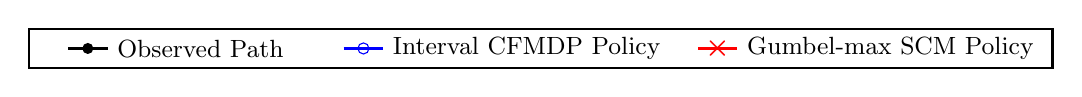
\begin{tikzpicture}[scale=1.0, every node/.style={scale=1.0}]
            \draw[thick, black] (-3, -0.25) rectangle (10, 0.25);
            %
            \draw[black, line width=1pt] (-2.5, 0.0) -- (-2,0.0);
            \fill[black] (-2.25,0.0) circle (2pt); %
            \node[right] at (-2,0.0) {\small Observed Path};
            
            %
            \draw[blue, line width=1pt] (1.0,0.0) -- (1.5,0.0);
            \node[draw=blue, circle, minimum size=4pt, inner sep=0pt] at (1.25,0.0) {}; %
            \node[right] at (1.5,0.0) {\small Interval CFMDP Policy};
            
            %
            \draw[red, line width=1pt] (5.5,0) -- (6,0);
            \node[red] at (5.75,0) {$\boldsymbol{\times}$}; %
            \node[right] at (6,0) {\small Gumbel-max SCM Policy};
        \end{tikzpicture}
    }\\
    %
    \subfigure[\footnotesize Lowest cumulative reward: Interval CFMDP ($312$), Gumbel-max SCM ($312$)]{%
        \resizebox{0.76\columnwidth}{!}{
             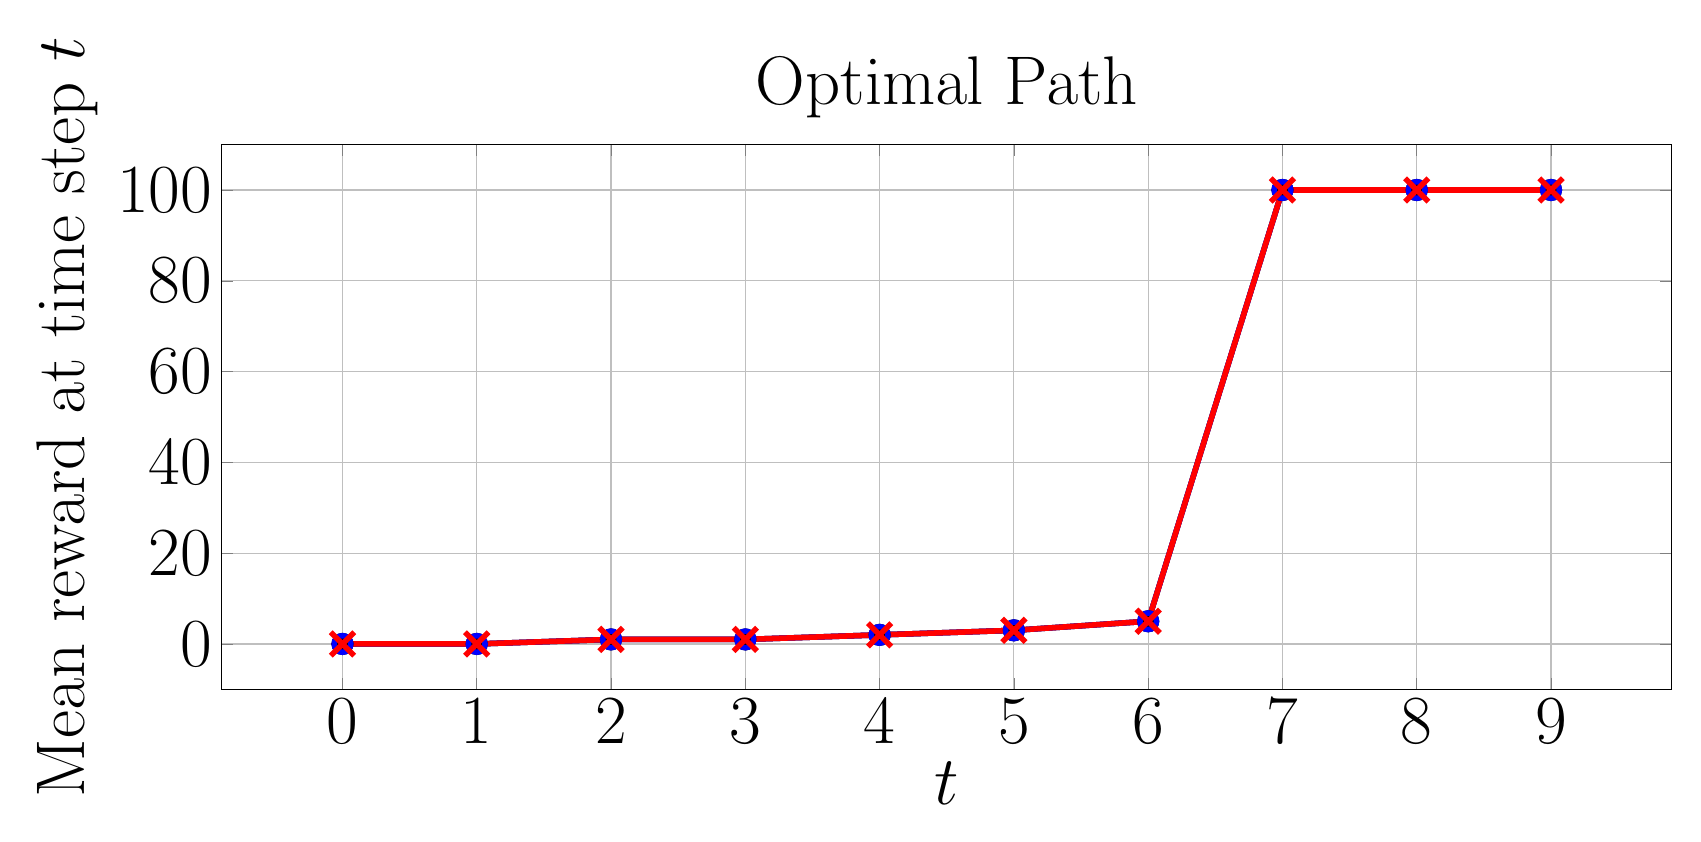
\begin{tikzpicture}
                \begin{axis}[
                    xlabel={$t$},
                    ylabel={Mean reward at time step $t$},
                    title={Optimal Path},
                    grid=both,
                    width=20cm, height=8.5cm,
                    every axis/.style={font=\Huge},
                    %
                ]
                \addplot[
                    color=black, %
                    mark=*, %
                    line width=2pt,
                    mark size=3pt,
                    error bars/.cd,
                    y dir=both, %
                    y explicit, %
                    error bar style={line width=1pt,solid},
                    error mark options={line width=1pt,mark size=4pt,rotate=90}
                ]
                coordinates {
                    (0, 0.0)  +- (0, 0.0)
                    (1, 0.0)  +- (0, 0.0) 
                    (2, 1.0)  +- (0, 0.0) 
                    (3, 1.0)  +- (0, 0.0)
                    (4, 2.0)  +- (0, 0.0)
                    (5, 3.0) +- (0, 0.0)
                    (6, 5.0) +- (0, 0.0)
                    (7, 100.0) +- (0, 0.0)
                    (8, 100.0) +- (0, 0.0)
                    (9, 100.0) +- (0, 0.0)
                };
                %
                \addplot[
                    color=blue, %
                    mark=o, %
                    line width=2pt,
                    mark size=3pt,
                    error bars/.cd,
                    y dir=both, %
                    y explicit, %
                    error bar style={line width=1pt,solid},
                    error mark options={line width=1pt,mark size=4pt,rotate=90}
                ]
                 coordinates {
                    (0, 0.0)  +- (0, 0.0)
                    (1, 0.0)  +- (0, 0.0) 
                    (2, 1.0)  +- (0, 0.0) 
                    (3, 1.0)  +- (0, 0.0)
                    (4, 2.0)  +- (0, 0.0)
                    (5, 3.0) +- (0, 0.0)
                    (6, 5.0) +- (0, 0.0)
                    (7, 100.0) +- (0, 0.0)
                    (8, 100.0) +- (0, 0.0)
                    (9, 100.0) +- (0, 0.0)
                };
                %
                \addplot[
                    color=red, %
                    mark=x, %
                    line width=2pt,
                    mark size=6pt,
                    error bars/.cd,
                    y dir=both, %
                    y explicit, %
                    error bar style={line width=1pt,solid},
                    error mark options={line width=1pt,mark size=4pt,rotate=90}
                ]
                coordinates {
                    (0, 0.0)  +- (0, 0.0)
                    (1, 0.0)  +- (0, 0.0) 
                    (2, 1.0)  +- (0, 0.0) 
                    (3, 1.0)  +- (0, 0.0)
                    (4, 2.0)  +- (0, 0.0)
                    (5, 3.0) +- (0, 0.0)
                    (6, 5.0) +- (0, 0.0)
                    (7, 100.0) +- (0, 0.0)
                    (8, 100.0) +- (0, 0.0)
                    (9, 100.0) +- (0, 0.0)
                };
                \end{axis}
            \end{tikzpicture}
         }
    }
    \hspace{1cm}
    \subfigure[\footnotesize Lowest cumulative reward: Interval CFMDP ($19$), Gumbel-max SCM ($-88$)]{%
         \resizebox{0.76\columnwidth}{!}{
            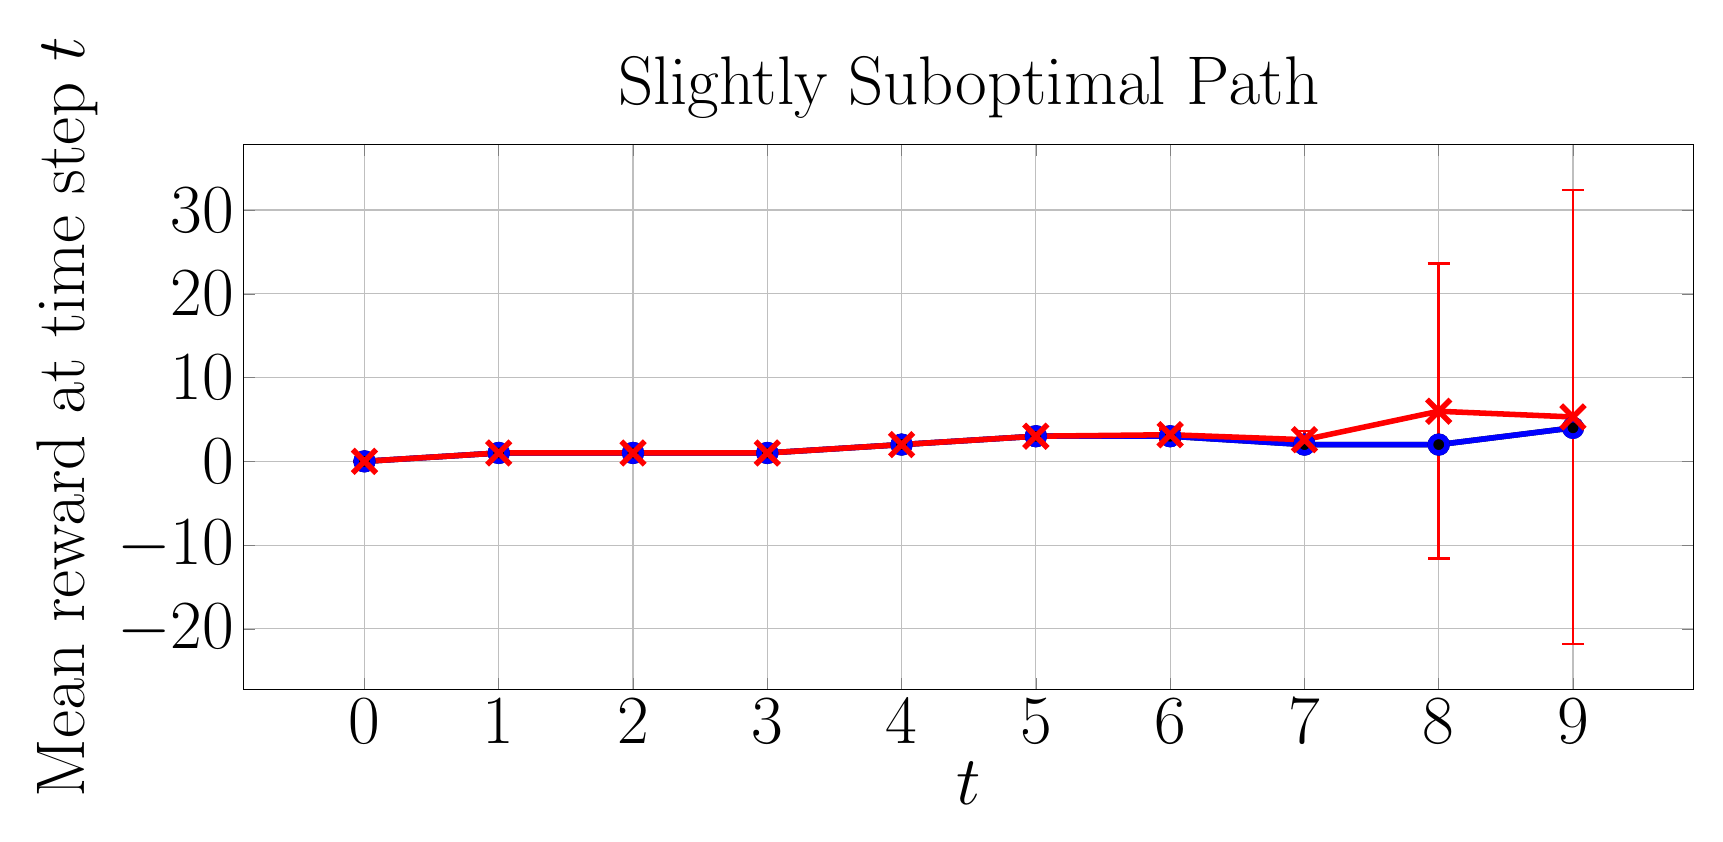
\begin{tikzpicture}
                \begin{axis}[
                    xlabel={$t$},
                    ylabel={Mean reward at time step $t$},
                    title={Slightly Suboptimal Path},
                    grid=both,
                    width=20cm, height=8.5cm,
                    every axis/.style={font=\Huge},
                    %
                ]
                \addplot[
                    color=black, %
                    mark=*, %
                    line width=2pt,
                    mark size=3pt,
                    error bars/.cd,
                    y dir=both, %
                    y explicit, %
                    error bar style={line width=1pt,solid},
                    error mark options={line width=1pt,mark size=4pt,rotate=90}
                ]
              coordinates {
                    (0, 0.0)  +- (0, 0.0)
                    (1, 1.0)  +- (0, 0.0) 
                    (2, 1.0)  +- (0, 0.0) 
                    (3, 1.0)  +- (0, 0.0)
                    (4, 2.0)  +- (0, 0.0)
                    (5, 3.0) +- (0, 0.0)
                    (6, 3.0) +- (0, 0.0)
                    (7, 2.0) +- (0, 0.0)
                    (8, 2.0) +- (0, 0.0)
                    (9, 4.0) +- (0, 0.0)
                };
                %
                \addplot[
                    color=blue, %
                    mark=o, %
                    line width=2pt,
                    mark size=3pt,
                    error bars/.cd,
                    y dir=both, %
                    y explicit, %
                    error bar style={line width=1pt,solid},
                    error mark options={line width=1pt,mark size=4pt,rotate=90}
                ]
              coordinates {
                    (0, 0.0)  +- (0, 0.0)
                    (1, 1.0)  +- (0, 0.0) 
                    (2, 1.0)  +- (0, 0.0) 
                    (3, 1.0)  +- (0, 0.0)
                    (4, 2.0)  +- (0, 0.0)
                    (5, 3.0) +- (0, 0.0)
                    (6, 3.0) +- (0, 0.0)
                    (7, 2.0) +- (0, 0.0)
                    (8, 2.0) +- (0, 0.0)
                    (9, 4.0) +- (0, 0.0)
                };
                %
                \addplot[
                    color=red, %
                    mark=x, %
                    line width=2pt,
                    mark size=6pt,
                    error bars/.cd,
                    y dir=both, %
                    y explicit, %
                    error bar style={line width=1pt,solid},
                    error mark options={line width=1pt,mark size=4pt,rotate=90}
                ]
                coordinates {
                    (0, 0.0)  +- (0, 0.0)
                    (1, 1.0)  +- (0, 0.0) 
                    (2, 1.0)  +- (0, 0.0) 
                    (3, 1.0)  +- (0, 0.0)
                    (4, 2.0)  += (0, 0.0)
                    (5, 3.0)  += (0, 0.0)
                    (6, 3.17847) += (0, 0.62606746) -= (0, 0.62606746)
                    (7, 2.5832885) += (0, 1.04598233) -= (0, 1.04598233)
                    (8, 5.978909) += (0, 17.60137623) -= (0, 17.60137623)
                    (9, 5.297059) += (0, 27.09227512) -= (0, 27.09227512)
                };
                \end{axis}
            \end{tikzpicture}
         }
    }\\[-1.5pt]
    \subfigure[\footnotesize Lowest cumulative reward: Interval CFMDP ($14$), Gumbel-max SCM ($-598$)]{%
         \resizebox{0.76\columnwidth}{!}{
             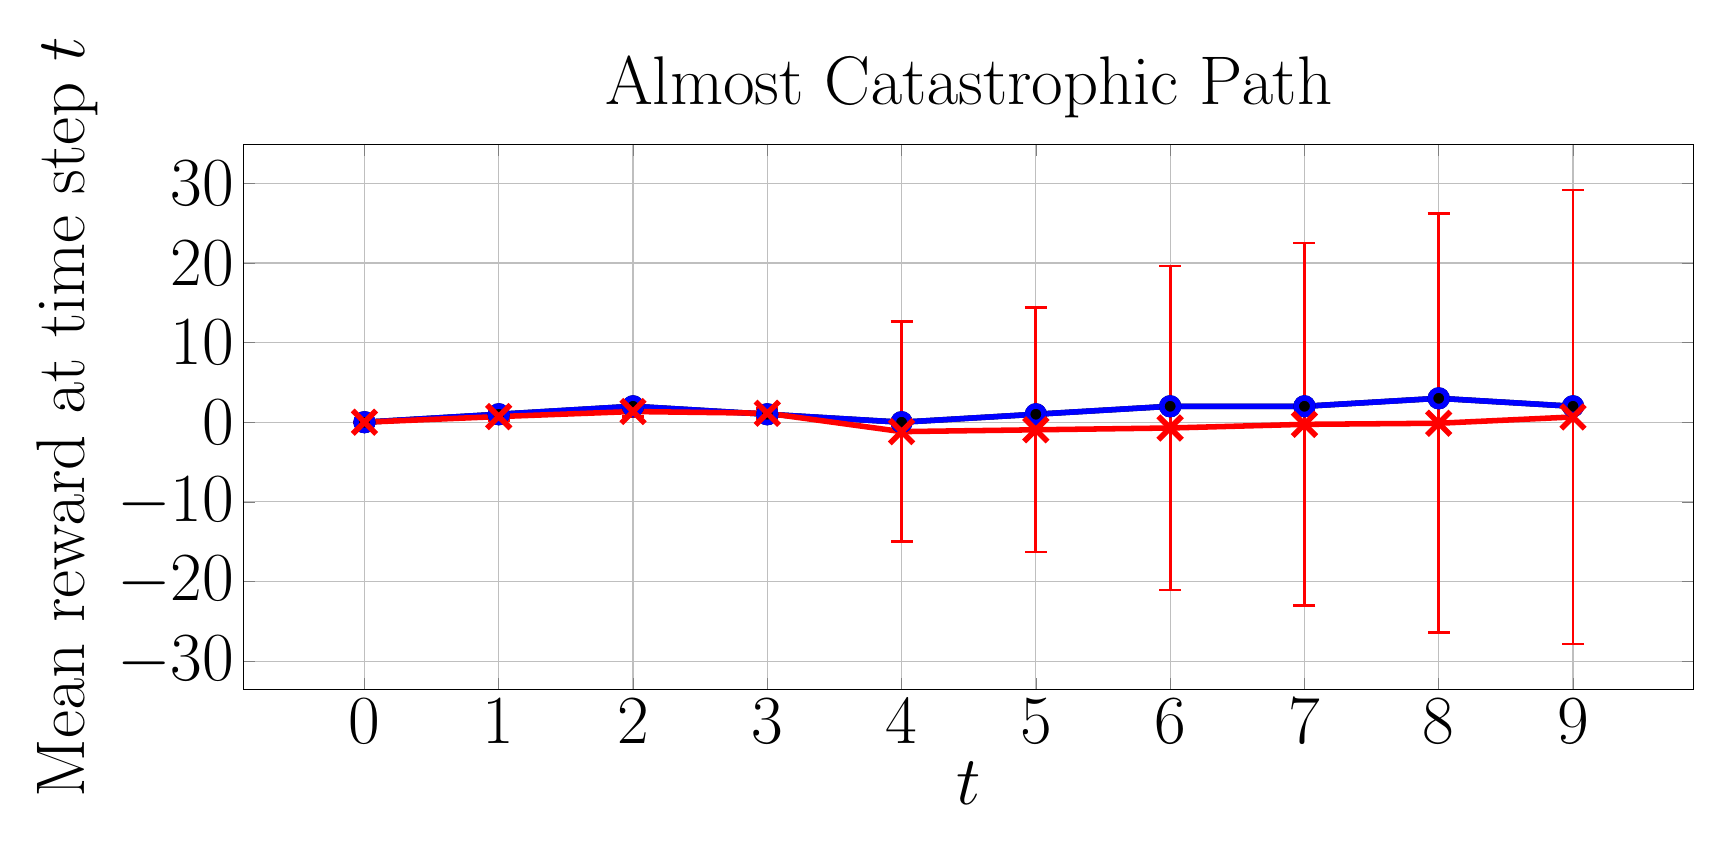
\begin{tikzpicture}
                \begin{axis}[
                    xlabel={$t$},
                    ylabel={Mean reward at time step $t$},
                    title={Almost Catastrophic Path},
                    grid=both,
                    width=20cm, height=8.5cm,
                    every axis/.style={font=\Huge},
                    %
                ]
                \addplot[
                    color=black, %
                    mark=*, %
                    line width=2pt,
                    mark size=3pt,
                    error bars/.cd,
                    y dir=both, %
                    y explicit, %
                    error bar style={line width=1pt,solid},
                    error mark options={line width=1pt,mark size=4pt,rotate=90}
                ]
                coordinates {
                    (0, 0.0)  +- (0, 0.0)
                    (1, 1.0)  +- (0, 0.0) 
                    (2, 2.0)  +- (0, 0.0) 
                    (3, 1.0)  +- (0, 0.0)
                    (4, 0.0)  +- (0, 0.0)
                    (5, 1.0) +- (0, 0.0)
                    (6, 2.0) +- (0, 0.0)
                    (7, 2.0) +- (0, 0.0)
                    (8, 3.0) +- (0, 0.0)
                    (9, 2.0) +- (0, 0.0)
                };
                %
                \addplot[
                    color=blue, %
                    mark=o, %
                    line width=2pt,
                    mark size=3pt,
                    error bars/.cd,
                    y dir=both, %
                    y explicit, %
                    error bar style={line width=1pt,solid},
                    error mark options={line width=1pt,mark size=4pt,rotate=90}
                ]
                coordinates {
                    (0, 0.0)  +- (0, 0.0)
                    (1, 1.0)  +- (0, 0.0) 
                    (2, 2.0)  +- (0, 0.0) 
                    (3, 1.0)  +- (0, 0.0)
                    (4, 0.0)  +- (0, 0.0)
                    (5, 1.0) +- (0, 0.0)
                    (6, 2.0) +- (0, 0.0)
                    (7, 2.0) +- (0, 0.0)
                    (8, 3.0) +- (0, 0.0)
                    (9, 2.0) +- (0, 0.0)
                };
                %
                \addplot[
                    color=red, %
                    mark=x, %
                    line width=2pt,
                    mark size=6pt,
                    error bars/.cd,
                    y dir=both, %
                    y explicit, %
                    error bar style={line width=1pt,solid},
                    error mark options={line width=1pt,mark size=4pt,rotate=90}
                ]
                coordinates {
                    (0, 0.0)  +- (0, 0.0)
                    (1, 0.7065655)  +- (0, 0.4553358) 
                    (2, 1.341673)  +- (0, 0.67091621) 
                    (3, 1.122926)  +- (0, 0.61281824)
                    (4, -1.1821935)  +- (0, 13.82444042)
                    (5, -0.952399)  +- (0, 15.35195457)
                    (6, -0.72672) +- (0, 20.33508414)
                    (7, -0.268983) +- (0, 22.77861454)
                    (8, -0.1310835) +- (0, 26.31013314)
                    (9, 0.65806) +- (0, 28.50670214)
                };
                %
            %
            %
            %
            %
            %
            %
            %
            %
            %
            %
            %
            %
            %
            %
            %
            %
            %
            %
                \end{axis}
            \end{tikzpicture}
         }
    }
    \hspace{1cm}
    \subfigure[\footnotesize Lowest cumulative reward: Interval CFMDP ($-698$), Gumbel-max SCM ($-698$)]{%
         \resizebox{0.76\columnwidth}{!}{
            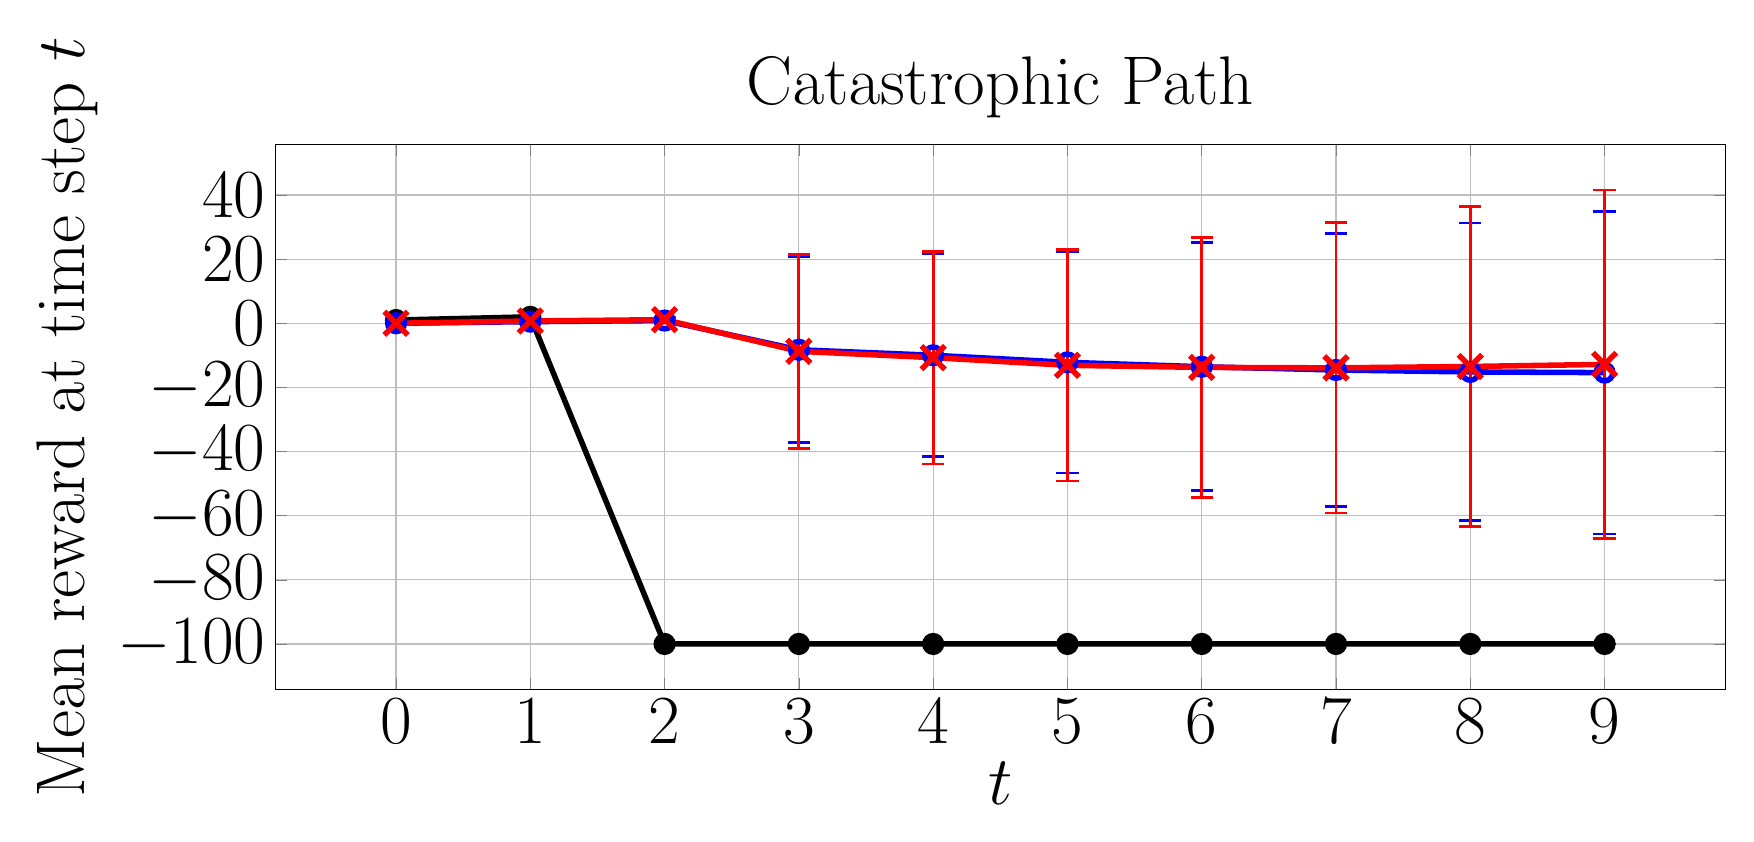
\begin{tikzpicture}
                \begin{axis}[
                    xlabel={$t$},
                    ylabel={Mean reward at time step $t$},
                    title={Catastrophic Path},
                    grid=both,
                    width=20cm, height=8.5cm,
                    every axis/.style={font=\Huge},
                    %
                ]
                \addplot[
                    color=black, %
                    mark=*, %
                    line width=2pt,
                    mark size=3pt,
                    error bars/.cd,
                    y dir=both, %
                    y explicit, %
                    error bar style={line width=1pt,solid},
                    error mark options={line width=1pt,mark size=4pt,rotate=90}
                ]
                coordinates {
                    (0, 1.0)  +- (0, 0.0)
                    (1, 2.0)  +- (0, 0.0) 
                    (2, -100.0)  +- (0, 0.0) 
                    (3, -100.0)  +- (0, 0.0)
                    (4, -100.0)  +- (0, 0.0)
                    (5, -100.0) +- (0, 0.0)
                    (6, -100.0) +- (0, 0.0)
                    (7, -100.0) +- (0, 0.0)
                    (8, -100.0) +- (0, 0.0)
                    (9, -100.0) +- (0, 0.0)
                };
                %
                \addplot[
                    color=blue, %
                    mark=o, %
                    line width=2pt,
                    mark size=3pt,
                    error bars/.cd,
                    y dir=both, %
                    y explicit, %
                    error bar style={line width=1pt,solid},
                    error mark options={line width=1pt,mark size=4pt,rotate=90}
                ]
                coordinates {
                    (0, 0.0)  +- (0, 0.0)
                    (1, 0.504814)  +- (0, 0.49997682) 
                    (2, 0.8439835)  +- (0, 0.76831917) 
                    (3, -8.2709165)  +- (0, 28.93656754)
                    (4, -9.981082)  +- (0, 31.66825363)
                    (5, -12.1776325) +- (0, 34.53463233)
                    (6, -13.556076) +- (0, 38.62845372)
                    (7, -14.574418) +- (0, 42.49603359)
                    (8, -15.1757075) +- (0, 46.41913968)
                    (9, -15.3900395) +- (0, 50.33563368)
                };
                %
                \addplot[
                    color=red, %
                    mark=x, %
                    line width=2pt,
                    mark size=6pt,
                    error bars/.cd,
                    y dir=both, %
                    y explicit, %
                    error bar style={line width=1pt,solid},
                    error mark options={line width=1pt,mark size=4pt,rotate=90}
                ]
                coordinates {
                    (0, 0.0)  +- (0, 0.0)
                    (1, 0.701873)  +- (0, 0.45743556) 
                    (2, 1.1227805)  +- (0, 0.73433129) 
                    (3, -8.7503255)  +- (0, 30.30257976)
                    (4, -10.722092)  +- (0, 33.17618589)
                    (5, -13.10721)  +- (0, 36.0648089)
                    (6, -13.7631645) +- (0, 40.56553451)
                    (7, -13.909043) +- (0, 45.23829402)
                    (8, -13.472517) +- (0, 49.96270296)
                    (9, -12.8278835) +- (0, 54.38618735)
                };
                %
            %
            %
            %
            %
            %
            %
            %
            %
            %
            %
            %
            %
            %
            %
            %
            %
            %
            %
                \end{axis}
            \end{tikzpicture}
         }
    }
    \caption{Average instant reward of CF paths induced by policies on GridWorld $p=0.4$.}
    \label{fig: reward p=0.4}
\end{figure*}

\subsection{Experimental Setup}
To compare policy performance, we measure the average rewards of counterfactual paths induced by our policy and the Gumbel-max policy by uniformly sampling $200$ counterfactual MDPs from the ICFMDP and generating $10,000$ counterfactual paths over each sampled CFMDP. \jl{Since the interval CFMDP depends on the observed path, we select $4$  paths of varying optimality to evaluate how the observed path impacts the performance of both policies: an optimal path, a slightly suboptimal path that could reach the optimal reward with a few changes, a catastrophic path that enters a catastrophic, terminal state with low reward, and an almost catastrophic path that was close to entering a catastrophic state.} When measuring the average probability bound widths and execution time needed to generate the ICFMDPs, we averaged over $20$ randomly generated observed paths
\footnote{Further training details are provided in Appendix \ref{app: training details}, and the code is provided at \href{https://github.com/ddv-lab/robust-cf-inference-in-MDPs}{https://github.com/ddv-lab/robust-cf-inference-in-MDPs}
%
%
.}.

\subsection{GridWorld}
\jl{The GridWorld MDP is a $4 \times 4$ grid where an agent must navigate from the top-left corner to the goal state in the bottom-right corner, avoiding a dangerous terminal state in the centre. At each time step, the agent can move up, down, left, or right, but there is a small probability (controlled by hyper-parameter $p$) of moving in an unintended direction. As the agent nears the goal, the reward for each state increases, culminating in a reward of $+100$ for reaching the goal. Entering the dangerous state results in a penalty of $-100$. We use two versions of GridWorld: a less stochastic version with $p=0.9$ (i.e., $90$\% chance of moving in the chosen direction) and a more stochastic version with $p=0.4$.}

\paragraph{GridWorld ($p=0.9$)}
When $p=0.9$, the counterfactual probability bounds are typically narrow (see Table \ref{tab:nonzero_probs} for average measurements). Consequently, as shown in Figure \ref{fig: reward p=0.9}, both policies are nearly identical and perform similarly well across the optimal, slightly suboptimal, and catastrophic paths.
%
However, for the almost catastrophic path, the interval CFMDP path is more conservative and follows the observed path more closely (as this is where the probability bounds are narrowest), which typically requires one additional step to reach the goal state than the Gumbel-max SCM policy.
%

\paragraph{GridWorld ($p=0.4$)}
\jl{When $p=0.4$, the GridWorld environment becomes more uncertain, increasing the risk of entering the dangerous state even if correct actions are chosen. Thus, as shown in Figure \ref{fig: reward p=0.4}, the interval CFMDP policy adopts a more conservative approach, avoiding deviation from the observed policy if it cannot guarantee higher counterfactual rewards (see the slightly suboptimal and almost catastrophic paths), whereas the Gumbel-max SCM is inconsistent: it can yield higher rewards, but also much lower rewards, reflected in the wide error bars.} For the catastrophic path, both policies must deviate from the observed path to achieve a higher reward and, in this case, perform similarly.
%
%
%
%
\subsection{Sepsis}
The Sepsis MDP \citep{oberst2019counterfactual} simulates trajectories of Sepsis patients. Each state consists of four vital signs (heart rate, blood pressure, oxygen concentration, and glucose levels), categorised as low, normal, or high.
and three treatments that can be toggled on/off at each time step (8 actions in total). Unlike \citet{oberst2019counterfactual}, we scale rewards based on the number of out-of-range vital signs, between $-1000$ (patient dies) and $1000$ (patient discharged). \jl{Like the GridWorld $p=0.4$ experiment, the Sepsis MDP is highly uncertain, as many states are equally likely to lead to optimal and poor outcomes. Thus, as shown in Figure \ref{fig: reward sepsis}, both policies follow the observed optimal and almost catastrophic paths to guarantee rewards are no worse than the observation.} However, improving the catastrophic path requires deviating from the observation. Here, the Gumbel-max SCM policy, on average, performs better than the interval CFMDP policy. But, since both policies have lower bounds clipped at $-1000$, neither policy reliably improves over the observation. In contrast, for the slightly suboptimal path, the interval CFMDP policy performs significantly better, shown by its higher lower bounds. 
Moreover, in these two cases, the worst-case counterfactual path generated by the interval CFMDP policy is better than that of the Gumbel-max SCM policy,
indicating its greater robustness.
%
\begin{figure*}
    \centering
     \resizebox{0.6\textwidth}{!}{
        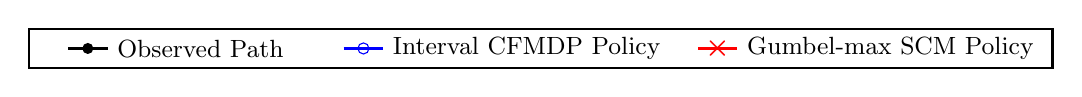
\begin{tikzpicture}[scale=1.0, every node/.style={scale=1.0}]
            \draw[thick, black] (-3, -0.25) rectangle (10, 0.25);
            %
            \draw[black, line width=1pt] (-2.5, 0.0) -- (-2,0.0);
            \fill[black] (-2.25,0.0) circle (2pt); %
            \node[right] at (-2,0.0) {\small Observed Path};
            
            %
            \draw[blue, line width=1pt] (1.0,0.0) -- (1.5,0.0);
            \node[draw=blue, circle, minimum size=4pt, inner sep=0pt] at (1.25,0.0) {}; %
            \node[right] at (1.5,0.0) {\small Interval CFMDP Policy};
            
            %
            \draw[red, line width=1pt] (5.5,0) -- (6,0);
            \node[red] at (5.75,0) {$\boldsymbol{\times}$}; %
            \node[right] at (6,0) {\small Gumbel-max SCM Policy};
        \end{tikzpicture}
    }\\
    \subfigure[\footnotesize Lowest cumulative reward: Interval CFMDP ($8000$), Gumbel-max SCM ($8000$)]{%
         \resizebox{0.76\columnwidth}{!}{
             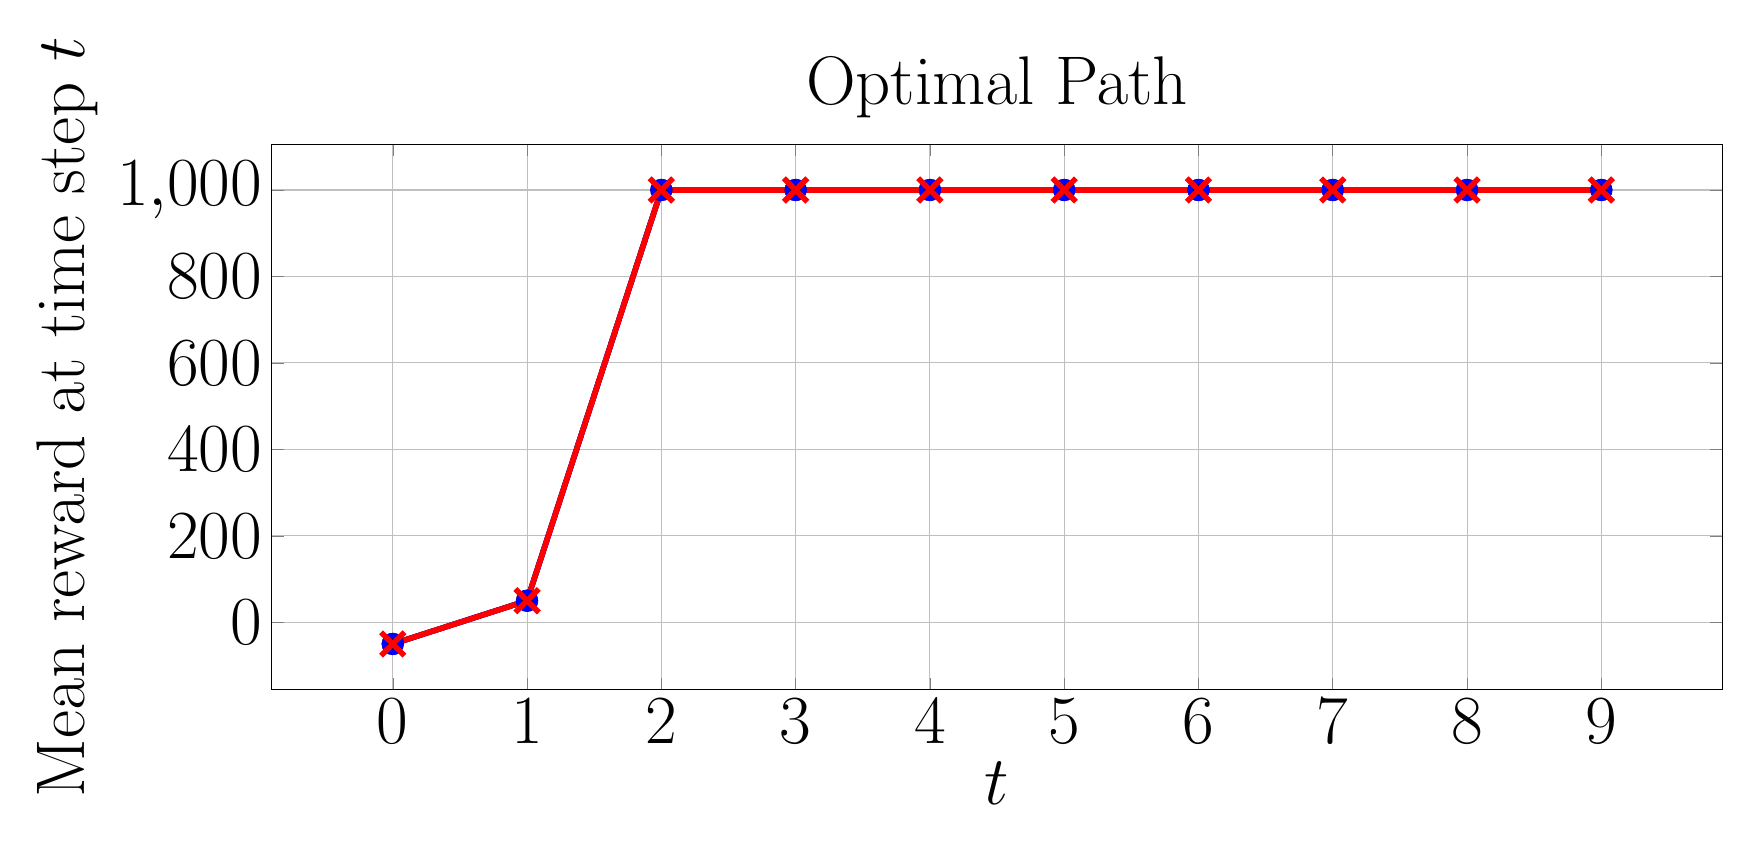
\begin{tikzpicture}
                \begin{axis}[
                    xlabel={$t$},
                    ylabel={Mean reward at time step $t$},
                    title={Optimal Path},
                    grid=both,
                    width=20cm, height=8.5cm,
                    every axis/.style={font=\Huge},
                    %
                ]
                \addplot[
                    color=black, %
                    mark=*, %
                    line width=2pt,
                    mark size=3pt,
                ]
                coordinates {
                    (0, -50.0)
                    (1, 50.0)
                    (2, 1000.0)
                    (3, 1000.0)
                    (4, 1000.0)
                    (5, 1000.0)
                    (6, 1000.0)
                    (7, 1000.0)
                    (8, 1000.0)
                    (9, 1000.0)
                };
                %
                \addplot[
                    color=blue, %
                    mark=o, %
                    line width=2pt,
                    mark size=3pt,
                    error bars/.cd,
                    y dir=both, %
                    y explicit, %
                    error bar style={line width=1pt,solid},
                    error mark options={line width=1pt,mark size=4pt,rotate=90}
                ]
                coordinates {
                    (0, -50.0)  +- (0, 0.0)
                    (1, 50.0)  +- (0, 0.0) 
                    (2, 1000.0)  +- (0, 0.0) 
                    (3, 1000.0)  +- (0, 0.0)
                    (4, 1000.0)  +- (0, 0.0)
                    (5, 1000.0) +- (0, 0.0)
                    (6, 1000.0) +- (0, 0.0)
                    (7, 1000.0) +- (0, 0.0)
                    (8, 1000.0) +- (0, 0.0)
                    (9, 1000.0) +- (0, 0.0)
                };
                %
                \addplot[
                    color=red, %
                    mark=x, %
                    line width=2pt,
                    mark size=6pt,
                    error bars/.cd,
                    y dir=both, %
                    y explicit, %
                    error bar style={line width=1pt,solid},
                    error mark options={line width=1pt,mark size=4pt,rotate=90}
                ]
                coordinates {
                    (0, -50.0)  +- (0, 0.0)
                    (1, 50.0)  +- (0, 0.0) 
                    (2, 1000.0)  +- (0, 0.0) 
                    (3, 1000.0)  +- (0, 0.0)
                    (4, 1000.0)  +- (0, 0.0)
                    (5, 1000.0) +- (0, 0.0)
                    (6, 1000.0) +- (0, 0.0)
                    (7, 1000.0) +- (0, 0.0)
                    (8, 1000.0) +- (0, 0.0)
                    (9, 1000.0) +- (0, 0.0)
                };
                %
                \end{axis}
            \end{tikzpicture}
         }
    }
    \hspace{1cm}
    \subfigure[\footnotesize Lowest cumulative reward: Interval CFMDP ($-5980$), Gumbel-max SCM ($-8000$)]{%
         \resizebox{0.76\columnwidth}{!}{
            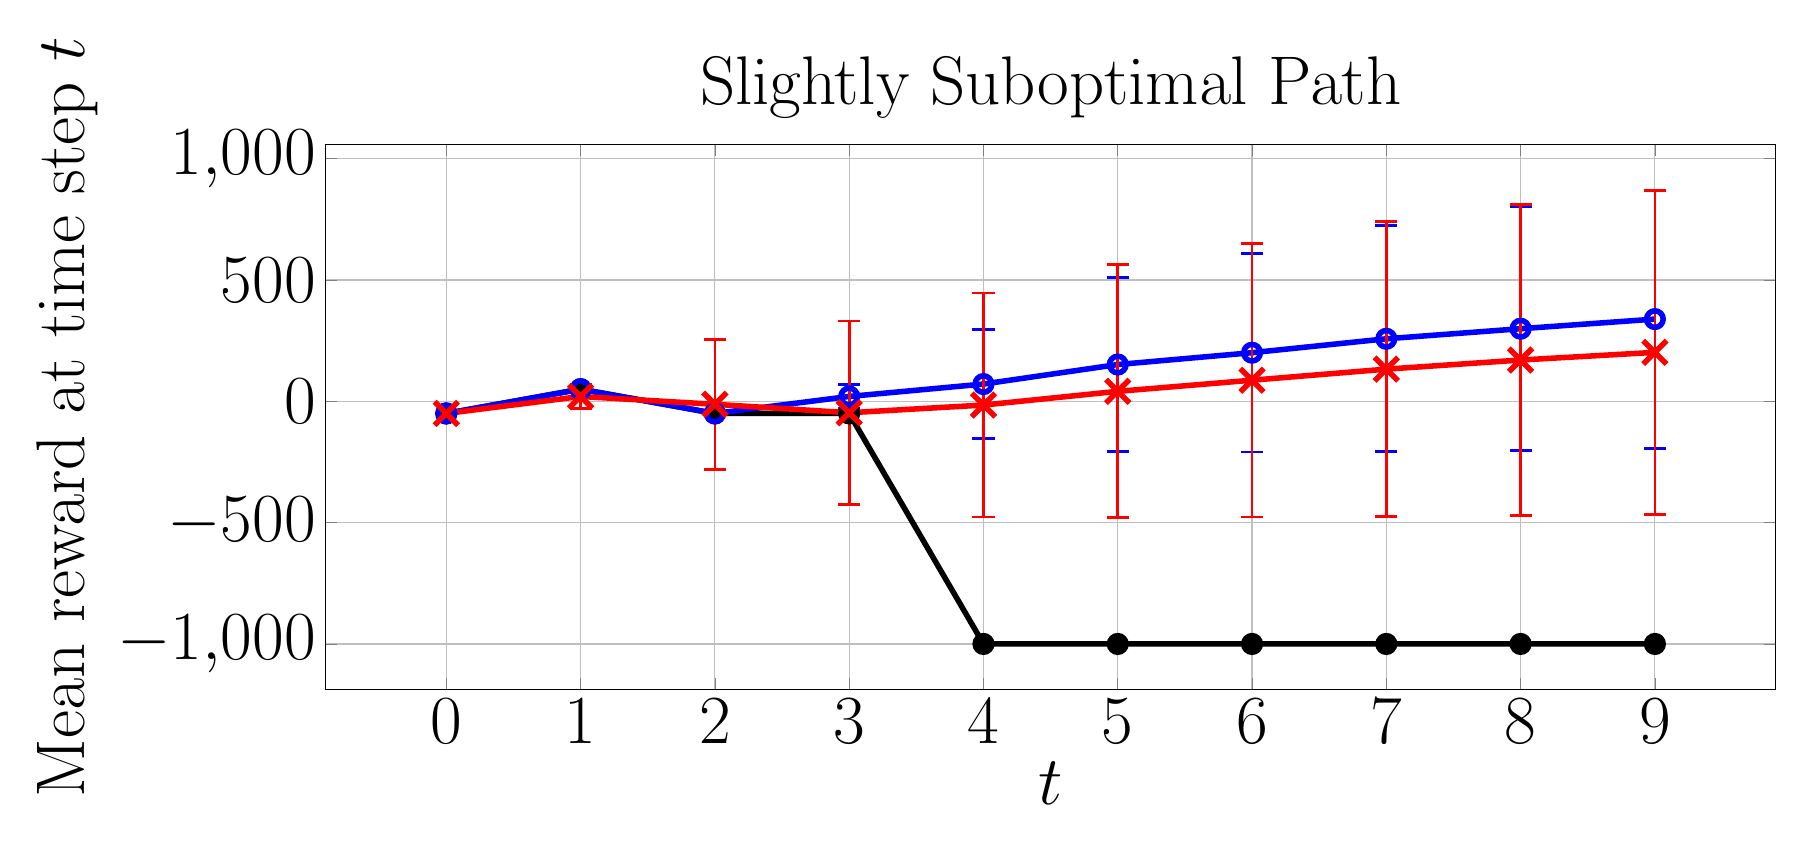
\begin{tikzpicture}
                \begin{axis}[
                    xlabel={$t$},
                    ylabel={Mean reward at time step $t$},
                    title={Slightly Suboptimal Path},
                    grid=both,
                    width=20cm, height=8.5cm,
                    every axis/.style={font=\Huge},
                    %
                ]
               \addplot[
                    color=black, %
                    mark=*, %
                    line width=2pt,
                    mark size=3pt,
                ]
                coordinates {
                    (0, -50.0)
                    (1, 50.0)
                    (2, -50.0)
                    (3, -50.0)
                    (4, -1000.0)
                    (5, -1000.0)
                    (6, -1000.0)
                    (7, -1000.0)
                    (8, -1000.0)
                    (9, -1000.0)
                };
                %
                \addplot[
                    color=blue, %
                    mark=o, %
                    line width=2pt,
                    mark size=3pt,
                    error bars/.cd,
                    y dir=both, %
                    y explicit, %
                    error bar style={line width=1pt,solid},
                    error mark options={line width=1pt,mark size=4pt,rotate=90}
                ]
                coordinates {
                    (0, -50.0)  +- (0, 0.0)
                    (1, 50.0)  +- (0, 0.0) 
                    (2, -50.0)  +- (0, 0.0) 
                    (3, 20.0631)  +- (0, 49.97539413)
                    (4, 71.206585)  +- (0, 226.02033693)
                    (5, 151.60797) +- (0, 359.23292559)
                    (6, 200.40593) +- (0, 408.86185176)
                    (7, 257.77948) +- (0, 466.10372804)
                    (8, 299.237465) +- (0, 501.82579506)
                    (9, 338.9129) +- (0, 532.06124996)
                };
                %
                \addplot[
                    color=red, %
                    mark=x, %
                    line width=2pt,
                    mark size=6pt,
                    error bars/.cd,
                    y dir=both, %
                    y explicit, %
                    error bar style={line width=1pt,solid},
                    error mark options={line width=1pt,mark size=4pt,rotate=90}
                ]
                coordinates {
                    (0, -50.0)  +- (0, 0.0)
                    (1, 20.00736)  +- (0, 49.99786741) 
                    (2, -12.282865)  +- (0, 267.598755) 
                    (3, -47.125995)  +- (0, 378.41755832)
                    (4, -15.381965)  +- (0, 461.77616558)
                    (5, 41.15459) +- (0, 521.53189262)
                    (6, 87.01595) +- (0, 564.22243126 )
                    (7, 132.62376) +- (0, 607.31338037)
                    (8, 170.168145) +- (0, 641.48013693)
                    (9, 201.813135) +- (0, 667.29441777)
                };
                %
                %
                %
                %
                %
                %
                %
                %
                %
                %
                %
                %
                %
                %
                %
                %
                %
                %
                %
                \end{axis}
            \end{tikzpicture}
         }
    }\\[-1.5pt]
    \subfigure[\footnotesize Lowest cumulative reward: Interval CFMDP ($100$), Gumbel-max SCM ($100$)]{%
         \resizebox{0.76\columnwidth}{!}{
             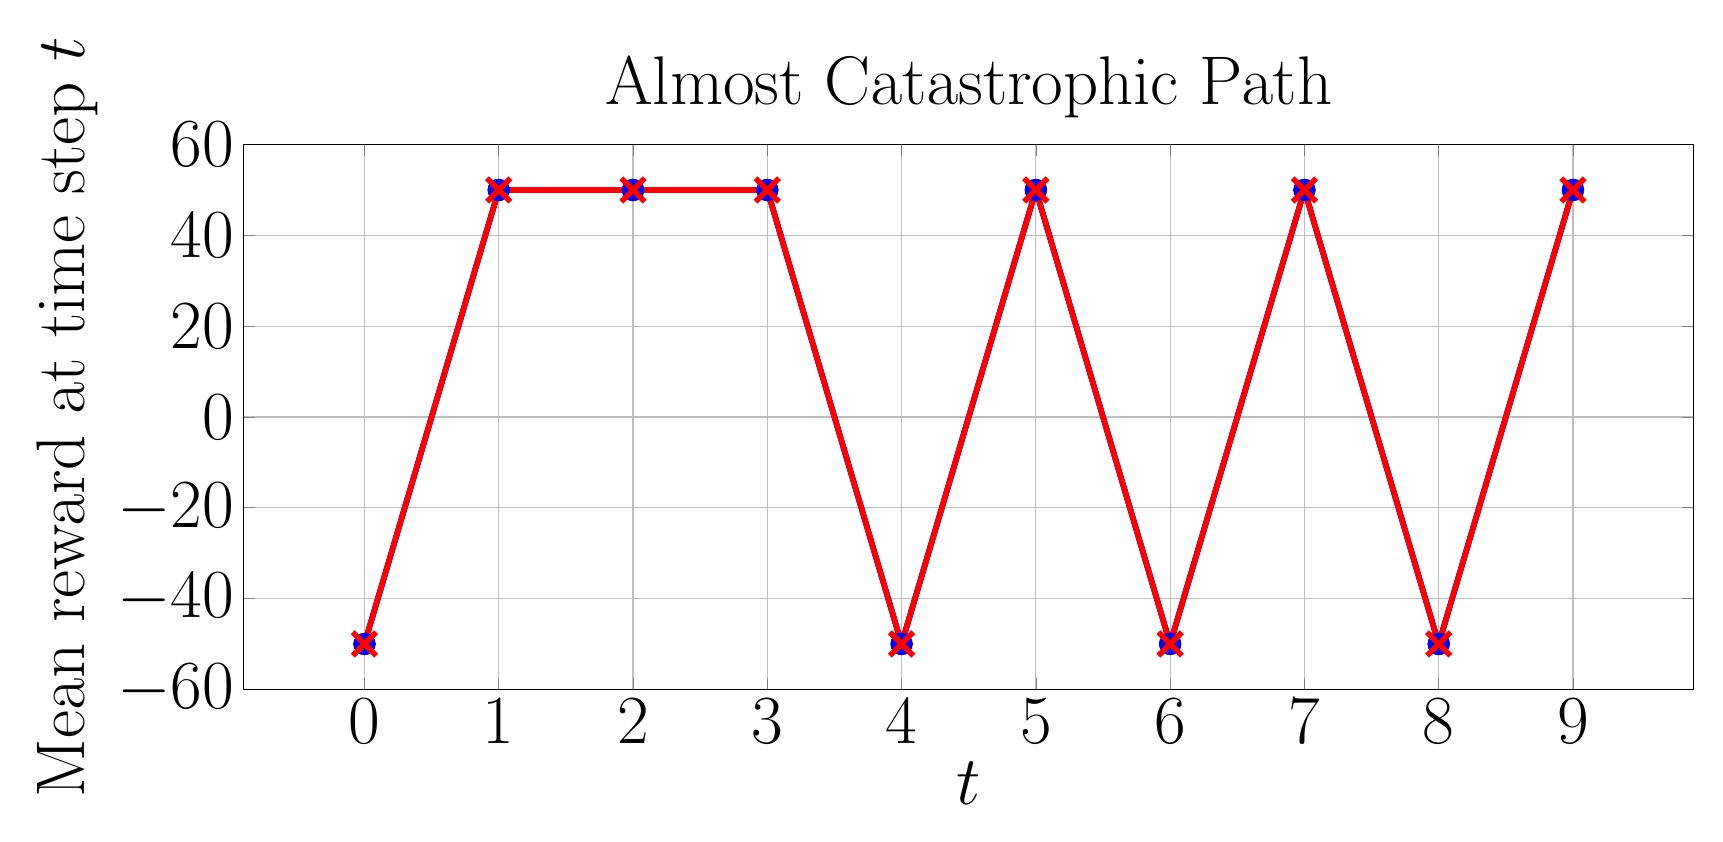
\begin{tikzpicture}
                \begin{axis}[
                    xlabel={$t$},
                    ylabel={Mean reward at time step $t$},
                    title={Almost Catastrophic Path},
                    grid=both,
                    every axis/.style={font=\Huge},
                    width=20cm, height=8.5cm,
                    %
                ]
               \addplot[
                    color=black, %
                    mark=*, %
                    line width=2pt,
                    mark size=3pt,
                ]
                coordinates {
                    (0, -50.0)
                    (1, 50.0)
                    (2, 50.0)
                    (3, 50.0)
                    (4, -50.0)
                    (5, 50.0)
                    (6, -50.0)
                    (7, 50.0)
                    (8, -50.0)
                    (9, 50.0)
                };
                %
                %
                \addplot[
                    color=blue, %
                    mark=o, %
                    line width=2pt,
                    mark size=3pt,
                    error bars/.cd,
                    y dir=both, %
                    y explicit, %
                    error bar style={line width=1pt,solid},
                    error mark options={line width=1pt,mark size=4pt,rotate=90}
                ]
                coordinates {
                    (0, -50.0)  +- (0, 0.0)
                    (1, 50.0)  +- (0, 0.0) 
                    (2, 50.0)  +- (0, 0.0) 
                    (3, 50.0)  +- (0, 0.0)
                    (4, -50.0)  +- (0, 0.0)
                    (5, 50.0) +- (0, 0.0)
                    (6, -50.0) +- (0, 0.0)
                    (7, 50.0) +- (0, 0.0)
                    (8, -50.0) +- (0, 0.0)
                    (9, 50.0) +- (0, 0.0)
                };
                %
                \addplot[
                    color=red, %
                    mark=x, %
                    line width=2pt,
                    mark size=6pt,
                    error bars/.cd,
                    y dir=both, %
                    y explicit, %
                    error bar style={line width=1pt,solid},
                    error mark options={line width=1pt,mark size=4pt,rotate=90}
                ]
                coordinates {
                    (0, -50.0)  +- (0, 0.0)
                    (1, 50.0)  +- (0, 0.0) 
                    (2, 50.0)  +- (0, 0.0) 
                    (3, 50.0)  +- (0, 0.0)
                    (4, -50.0)  +- (0, 0.0)
                    (5, 50.0) +- (0, 0.0)
                    (6, -50.0) +- (0, 0.0)
                    (7, 50.0) +- (0, 0.0)
                    (8, -50.0) +- (0, 0.0)
                    (9, 50.0) +- (0, 0.0)
                };
                %
                %
                %
                %
                %
                %
                %
                %
                %
                %
                %
                %
                %
                %
                %
                %
                %
                %
                %
                \end{axis}
            \end{tikzpicture}
         }
    }
    \hspace{1cm}
    \subfigure[\footnotesize Lowest cumulative reward: Interval CFMDP ($-7150$), Gumbel-max SCM ($-9050$)]{%
         \resizebox{0.76\columnwidth}{!}{
            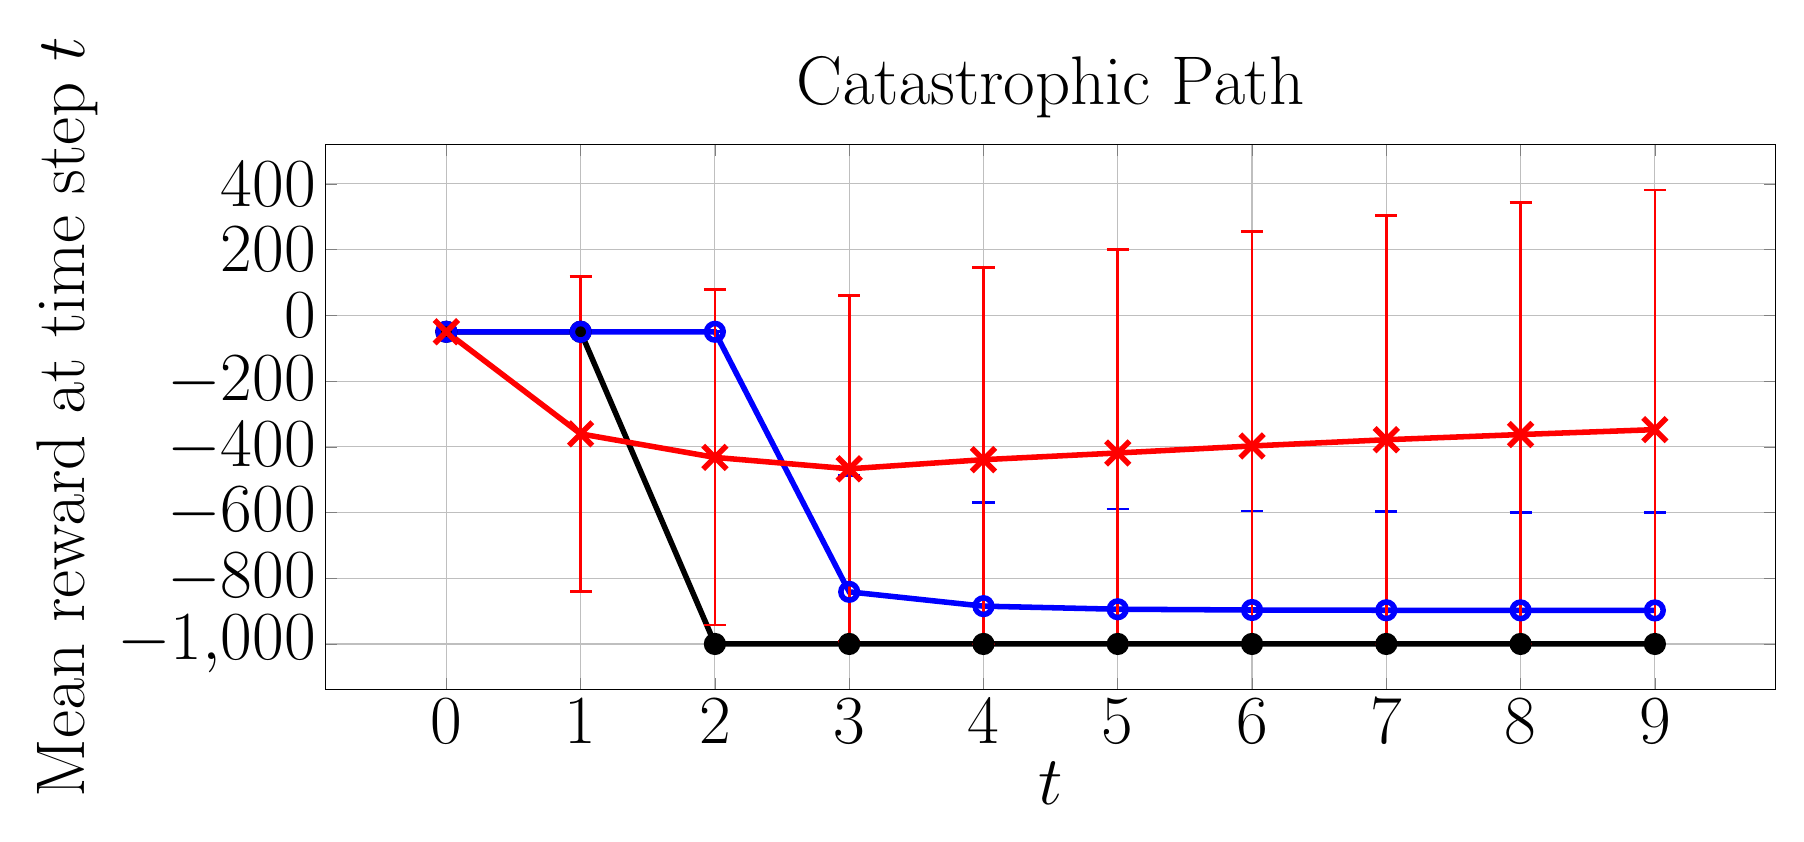
\begin{tikzpicture}
                \begin{axis}[
                    xlabel={$t$},
                    ylabel={Mean reward at time step $t$},
                    title={Catastrophic Path},
                    grid=both,
                    width=20cm, height=8.5cm,
                    every axis/.style={font=\Huge},
                    %
                ]
               \addplot[
                    color=black, %
                    mark=*, %
                    line width=2pt,
                    mark size=3pt,
                ]
                coordinates {
                    (0, -50.0)
                    (1, -50.0)
                    (2, -1000.0)
                    (3, -1000.0)
                    (4, -1000.0)
                    (5, -1000.0)
                    (6, -1000.0)
                    (7, -1000.0)
                    (8, -1000.0)
                    (9, -1000.0)
                };
                %
                %
                \addplot[
                    color=blue, %
                    mark=o, %
                    line width=2pt,
                    mark size=3pt,
                    error bars/.cd,
                    y dir=both, %
                    y explicit, %
                    error bar style={line width=1pt,solid},
                    error mark options={line width=1pt,mark size=4pt,rotate=90}
                ]
                coordinates {
                    (0, -50.0)  +- (0, 0.0)
                    (1, -50.0)  +- (0, 0.0) 
                    (2, -50.0)  +- (0, 0.0) 
                    (3, -841.440725)  += (0, 354.24605512) -= (0, 158.559275)
                    (4, -884.98225)  += (0, 315.37519669) -= (0, 115.01775)
                    (5, -894.330425) += (0, 304.88572805) -= (0, 105.669575)
                    (6, -896.696175) += (0, 301.19954514) -= (0, 103.303825)
                    (7, -897.4635) += (0, 299.61791279) -= (0, 102.5365)
                    (8, -897.77595) += (0, 298.80392585) -= (0, 102.22405)
                    (9, -897.942975) += (0, 298.32920557) -= (0, 102.057025)
                };
                %
                \addplot[
                    color=red, %
                    mark=x, %
                    line width=2pt,
                    mark size=6pt,
                    error bars/.cd,
                    y dir=both, %
                    y explicit, %
                    error bar style={line width=1pt,solid},
                    error mark options={line width=1pt,mark size=4pt,rotate=90}
                ]
            coordinates {
                    (0, -50.0)  +- (0, 0.0)
                    (1, -360.675265)  +- (0, 479.39812699) 
                    (2, -432.27629)  +- (0, 510.38620897) 
                    (3, -467.029545)  += (0, 526.36009628) -= (0, 526.36009628)
                    (4, -439.17429)  += (0, 583.96638919) -= (0, 560.82571)
                    (5, -418.82704) += (0, 618.43027478) -= (0, 581.17296)
                    (6, -397.464895) += (0, 652.67322574) -= (0, 602.535105)
                    (7, -378.49052) += (0, 682.85407033) -= (0, 621.50948)
                    (8, -362.654195) += (0, 707.01412023) -= (0, 637.345805)
                    (9, -347.737935) += (0, 729.29076479) -= (0, 652.262065)
                };
                %
                %
                %
                %
                %
                %
                %
                %
                %
                %
                %
                %
                %
                %
                %
                %
                %
                %
                %
                \end{axis}
            \end{tikzpicture}
         }
    }
    \caption{Average instant reward of CF paths induced by policies on Sepsis.}
    \label{fig: reward sepsis}
\end{figure*}

%
%
%
\subsection{Interval CFMDP Bounds}
%
%
Table \ref{tab:nonzero_probs} presents the mean counterfactual probability bound widths (excluding transitions where the upper bound is $0$) for each MDP, averaged over 20 observed paths. We compare the bounds under counterfactual stability (CS) and monotonicity (M) assumptions, CS alone, and no assumptions. This shows that the assumptions marginally reduce the bound widths, indicating the assumptions tighten the bounds without excluding too many causal models, as intended.
\renewcommand{\arraystretch}{1}

\begin{table}
\centering
\caption{Mean width of counterfactual probability bounds}
\resizebox{0.8\columnwidth}{!}{%
\begin{tabular}{|c|c|c|c|}
\hline
\multirow{2}{*}{\textbf{Environment}} & \multicolumn{3}{c|}{\textbf{Assumptions}} \\ \cline{2-4}
 & \textbf{CS + M} & \textbf{CS} & \textbf{None\tablefootnote{\jl{Equivalent to \citet{li2024probabilities}'s bounds (see Section \ref{sec: equivalence with Li}).}}} \\ \hline
\textbf{GridWorld} ($p=0.9$) & 0.0817 & 0.0977 & 0.100 \\ \hline
\textbf{GridWorld} ($p=0.4$) & 0.552  & 0.638  & 0.646 \\ \hline
\textbf{Sepsis} & 0.138 & 0.140 & 0.140 \\ \hline
\end{tabular}
}
\label{tab:nonzero_probs}
\end{table}


\subsection{Execution Times}
Table \ref{tab: times} compares the average time needed to generate the interval CFMDP vs.\ the Gumbel-max SCM CFMDP for 20 observations.
The GridWorld algorithms were run single-threaded, while the Sepsis experiments were run in parallel.
Generating the interval CFMDP is significantly faster as it uses exact analytical bounds, whereas the Gumbel-max CFMDP requires sampling from the Gumbel distribution to estimate counterfactual transition probabilities. \jl{Since constructing the counterfactual MDP models is the main bottleneck in both approaches, ours is more efficient overall and suitable for larger MDPs.}
\begin{table}
\centering
\caption{Mean execution time to generate CFMDPs}
\resizebox{0.99\columnwidth}{!}{%
\begin{tabular}{|c|c|c|}
\hline
\multirow{2}{*}{\textbf{Environment}} & \multicolumn{2}{c|}{\textbf{Mean Execution Time (s)}} \\ \cline{2-3} 
                                      & \textbf{Interval CFMDP} & \textbf{Gumbel-max CFMDP} \\ \hline
\textbf{GridWorld ($p=0.9$) }                  & 0.261                   & 56.1                      \\ \hline
\textbf{GridWorld ($p=0.4$)  }                 & 0.336                   & 54.5                      \\ \hline
\textbf{Sepsis}                                 & 688                     & 2940                      \\ \hline
\end{tabular}%
}
\label{tab: times}
\end{table}

\putsec{related}{Related Work}

\noindent \textbf{Efficient Radiance Field Rendering.}
%
The introduction of Neural Radiance Fields (NeRF)~\cite{mil:sri20} has
generated significant interest in efficient 3D scene representation and
rendering for radiance fields.
%
Over the past years, there has been a large amount of research aimed at
accelerating NeRFs through algorithmic or software
optimizations~\cite{mul:eva22,fri:yu22,che:fun23,sun:sun22}, and the
development of hardware
accelerators~\cite{lee:cho23,li:li23,son:wen23,mub:kan23,fen:liu24}.
%
The state-of-the-art method, 3D Gaussian splatting~\cite{ker:kop23}, has
further fueled interest in accelerating radiance field
rendering~\cite{rad:ste24,lee:lee24,nie:stu24,lee:rho24,ham:mel24} as it
employs rasterization primitives that can be rendered much faster than NeRFs.
%
However, previous research focused on software graphics rendering on
programmable cores or building dedicated hardware accelerators. In contrast,
\name{} investigates the potential of efficient radiance field rendering while
utilizing fixed-function units in graphics hardware.
%
To our knowledge, this is the first work that assesses the performance
implications of rendering Gaussian-based radiance fields on the hardware
graphics pipeline with software and hardware optimizations.

%%%%%%%%%%%%%%%%%%%%%%%%%%%%%%%%%%%%%%%%%%%%%%%%%%%%%%%%%%%%%%%%%%%%%%%%%%
\myparagraph{Enhancing Graphics Rendering Hardware.}
%
The performance advantage of executing graphics rendering on either
programmable shader cores or fixed-function units varies depending on the
rendering methods and hardware designs.
%
Previous studies have explored the performance implication of graphics hardware
design by developing simulation infrastructures for graphics
workloads~\cite{bar:gon06,gub:aam19,tin:sax23,arn:par13}.
%
Additionally, several studies have aimed to improve the performance of
special-purpose hardware such as ray tracing units in graphics
hardware~\cite{cho:now23,liu:cha21} and proposed hardware accelerators for
graphics applications~\cite{lu:hua17,ram:gri09}.
%
In contrast to these works, which primarily evaluate traditional graphics
workloads, our work focuses on improving the performance of volume rendering
workloads, such as Gaussian splatting, which require blending a huge number of
fragments per pixel.

%%%%%%%%%%%%%%%%%%%%%%%%%%%%%%%%%%%%%%%%%%%%%%%%%%%%%%%%%%%%%%%%%%%%%%%%%%
%
In the context of multi-sample anti-aliasing, prior work proposed reducing the
amount of redundant shading by merging fragments from adjacent triangles in a
mesh at the quad granularity~\cite{fat:bou10}.
%
While both our work and quad-fragment merging (QFM)~\cite{fat:bou10} aim to
reduce operations by merging quads, our proposed technique differs from QFM in
many aspects.
%
Our method aims to blend \emph{overlapping primitives} along the depth
direction and applies to quads from any primitive. In contrast, QFM merges quad
fragments from small (e.g., pixel-sized) triangles that \emph{share} an edge
(i.e., \emph{connected}, \emph{non-overlapping} triangles).
%
As such, QFM is not applicable to the scenes consisting of a number of
unconnected transparent triangles, such as those in 3D Gaussian splatting.
%
In addition, our method computes the \emph{exact} color for each pixel by
offloading blending operations from ROPs to shader units, whereas QFM
\emph{approximates} pixel colors by using the color from one triangle when
multiple triangles are merged into a single quad.


\section{Conclusion}
In this work, we propose a simple yet effective approach, called SMILE, for graph few-shot learning with fewer tasks. Specifically, we introduce a novel dual-level mixup strategy, including within-task and across-task mixup, for enriching the diversity of nodes within each task and the diversity of tasks. Also, we incorporate the degree-based prior information to learn expressive node embeddings. Theoretically, we prove that SMILE effectively enhances the model's generalization performance. Empirically, we conduct extensive experiments on multiple benchmarks and the results suggest that SMILE significantly outperforms other baselines, including both in-domain and cross-domain few-shot settings.


\balance
% \bibliographystyle{ACM-Reference-Format}
\bibliographystyle{IEEEtran}
\bibliography{sigproc}

% \appendix
\subsection{Lloyd-Max Algorithm}
\label{subsec:Lloyd-Max}
For a given quantization bitwidth $B$ and an operand $\bm{X}$, the Lloyd-Max algorithm finds $2^B$ quantization levels $\{\hat{x}_i\}_{i=1}^{2^B}$ such that quantizing $\bm{X}$ by rounding each scalar in $\bm{X}$ to the nearest quantization level minimizes the quantization MSE. 

The algorithm starts with an initial guess of quantization levels and then iteratively computes quantization thresholds $\{\tau_i\}_{i=1}^{2^B-1}$ and updates quantization levels $\{\hat{x}_i\}_{i=1}^{2^B}$. Specifically, at iteration $n$, thresholds are set to the midpoints of the previous iteration's levels:
\begin{align*}
    \tau_i^{(n)}=\frac{\hat{x}_i^{(n-1)}+\hat{x}_{i+1}^{(n-1)}}2 \text{ for } i=1\ldots 2^B-1
\end{align*}
Subsequently, the quantization levels are re-computed as conditional means of the data regions defined by the new thresholds:
\begin{align*}
    \hat{x}_i^{(n)}=\mathbb{E}\left[ \bm{X} \big| \bm{X}\in [\tau_{i-1}^{(n)},\tau_i^{(n)}] \right] \text{ for } i=1\ldots 2^B
\end{align*}
where to satisfy boundary conditions we have $\tau_0=-\infty$ and $\tau_{2^B}=\infty$. The algorithm iterates the above steps until convergence.

Figure \ref{fig:lm_quant} compares the quantization levels of a $7$-bit floating point (E3M3) quantizer (left) to a $7$-bit Lloyd-Max quantizer (right) when quantizing a layer of weights from the GPT3-126M model at a per-tensor granularity. As shown, the Lloyd-Max quantizer achieves substantially lower quantization MSE. Further, Table \ref{tab:FP7_vs_LM7} shows the superior perplexity achieved by Lloyd-Max quantizers for bitwidths of $7$, $6$ and $5$. The difference between the quantizers is clear at 5 bits, where per-tensor FP quantization incurs a drastic and unacceptable increase in perplexity, while Lloyd-Max quantization incurs a much smaller increase. Nevertheless, we note that even the optimal Lloyd-Max quantizer incurs a notable ($\sim 1.5$) increase in perplexity due to the coarse granularity of quantization. 

\begin{figure}[h]
  \centering
  \includegraphics[width=0.7\linewidth]{sections/figures/LM7_FP7.pdf}
  \caption{\small Quantization levels and the corresponding quantization MSE of Floating Point (left) vs Lloyd-Max (right) Quantizers for a layer of weights in the GPT3-126M model.}
  \label{fig:lm_quant}
\end{figure}

\begin{table}[h]\scriptsize
\begin{center}
\caption{\label{tab:FP7_vs_LM7} \small Comparing perplexity (lower is better) achieved by floating point quantizers and Lloyd-Max quantizers on a GPT3-126M model for the Wikitext-103 dataset.}
\begin{tabular}{c|cc|c}
\hline
 \multirow{2}{*}{\textbf{Bitwidth}} & \multicolumn{2}{|c|}{\textbf{Floating-Point Quantizer}} & \textbf{Lloyd-Max Quantizer} \\
 & Best Format & Wikitext-103 Perplexity & Wikitext-103 Perplexity \\
\hline
7 & E3M3 & 18.32 & 18.27 \\
6 & E3M2 & 19.07 & 18.51 \\
5 & E4M0 & 43.89 & 19.71 \\
\hline
\end{tabular}
\end{center}
\end{table}

\subsection{Proof of Local Optimality of LO-BCQ}
\label{subsec:lobcq_opt_proof}
For a given block $\bm{b}_j$, the quantization MSE during LO-BCQ can be empirically evaluated as $\frac{1}{L_b}\lVert \bm{b}_j- \bm{\hat{b}}_j\rVert^2_2$ where $\bm{\hat{b}}_j$ is computed from equation (\ref{eq:clustered_quantization_definition}) as $C_{f(\bm{b}_j)}(\bm{b}_j)$. Further, for a given block cluster $\mathcal{B}_i$, we compute the quantization MSE as $\frac{1}{|\mathcal{B}_{i}|}\sum_{\bm{b} \in \mathcal{B}_{i}} \frac{1}{L_b}\lVert \bm{b}- C_i^{(n)}(\bm{b})\rVert^2_2$. Therefore, at the end of iteration $n$, we evaluate the overall quantization MSE $J^{(n)}$ for a given operand $\bm{X}$ composed of $N_c$ block clusters as:
\begin{align*}
    \label{eq:mse_iter_n}
    J^{(n)} = \frac{1}{N_c} \sum_{i=1}^{N_c} \frac{1}{|\mathcal{B}_{i}^{(n)}|}\sum_{\bm{v} \in \mathcal{B}_{i}^{(n)}} \frac{1}{L_b}\lVert \bm{b}- B_i^{(n)}(\bm{b})\rVert^2_2
\end{align*}

At the end of iteration $n$, the codebooks are updated from $\mathcal{C}^{(n-1)}$ to $\mathcal{C}^{(n)}$. However, the mapping of a given vector $\bm{b}_j$ to quantizers $\mathcal{C}^{(n)}$ remains as  $f^{(n)}(\bm{b}_j)$. At the next iteration, during the vector clustering step, $f^{(n+1)}(\bm{b}_j)$ finds new mapping of $\bm{b}_j$ to updated codebooks $\mathcal{C}^{(n)}$ such that the quantization MSE over the candidate codebooks is minimized. Therefore, we obtain the following result for $\bm{b}_j$:
\begin{align*}
\frac{1}{L_b}\lVert \bm{b}_j - C_{f^{(n+1)}(\bm{b}_j)}^{(n)}(\bm{b}_j)\rVert^2_2 \le \frac{1}{L_b}\lVert \bm{b}_j - C_{f^{(n)}(\bm{b}_j)}^{(n)}(\bm{b}_j)\rVert^2_2
\end{align*}

That is, quantizing $\bm{b}_j$ at the end of the block clustering step of iteration $n+1$ results in lower quantization MSE compared to quantizing at the end of iteration $n$. Since this is true for all $\bm{b} \in \bm{X}$, we assert the following:
\begin{equation}
\begin{split}
\label{eq:mse_ineq_1}
    \tilde{J}^{(n+1)} &= \frac{1}{N_c} \sum_{i=1}^{N_c} \frac{1}{|\mathcal{B}_{i}^{(n+1)}|}\sum_{\bm{b} \in \mathcal{B}_{i}^{(n+1)}} \frac{1}{L_b}\lVert \bm{b} - C_i^{(n)}(b)\rVert^2_2 \le J^{(n)}
\end{split}
\end{equation}
where $\tilde{J}^{(n+1)}$ is the the quantization MSE after the vector clustering step at iteration $n+1$.

Next, during the codebook update step (\ref{eq:quantizers_update}) at iteration $n+1$, the per-cluster codebooks $\mathcal{C}^{(n)}$ are updated to $\mathcal{C}^{(n+1)}$ by invoking the Lloyd-Max algorithm \citep{Lloyd}. We know that for any given value distribution, the Lloyd-Max algorithm minimizes the quantization MSE. Therefore, for a given vector cluster $\mathcal{B}_i$ we obtain the following result:

\begin{equation}
    \frac{1}{|\mathcal{B}_{i}^{(n+1)}|}\sum_{\bm{b} \in \mathcal{B}_{i}^{(n+1)}} \frac{1}{L_b}\lVert \bm{b}- C_i^{(n+1)}(\bm{b})\rVert^2_2 \le \frac{1}{|\mathcal{B}_{i}^{(n+1)}|}\sum_{\bm{b} \in \mathcal{B}_{i}^{(n+1)}} \frac{1}{L_b}\lVert \bm{b}- C_i^{(n)}(\bm{b})\rVert^2_2
\end{equation}

The above equation states that quantizing the given block cluster $\mathcal{B}_i$ after updating the associated codebook from $C_i^{(n)}$ to $C_i^{(n+1)}$ results in lower quantization MSE. Since this is true for all the block clusters, we derive the following result: 
\begin{equation}
\begin{split}
\label{eq:mse_ineq_2}
     J^{(n+1)} &= \frac{1}{N_c} \sum_{i=1}^{N_c} \frac{1}{|\mathcal{B}_{i}^{(n+1)}|}\sum_{\bm{b} \in \mathcal{B}_{i}^{(n+1)}} \frac{1}{L_b}\lVert \bm{b}- C_i^{(n+1)}(\bm{b})\rVert^2_2  \le \tilde{J}^{(n+1)}   
\end{split}
\end{equation}

Following (\ref{eq:mse_ineq_1}) and (\ref{eq:mse_ineq_2}), we find that the quantization MSE is non-increasing for each iteration, that is, $J^{(1)} \ge J^{(2)} \ge J^{(3)} \ge \ldots \ge J^{(M)}$ where $M$ is the maximum number of iterations. 
%Therefore, we can say that if the algorithm converges, then it must be that it has converged to a local minimum. 
\hfill $\blacksquare$


\begin{figure}
    \begin{center}
    \includegraphics[width=0.5\textwidth]{sections//figures/mse_vs_iter.pdf}
    \end{center}
    \caption{\small NMSE vs iterations during LO-BCQ compared to other block quantization proposals}
    \label{fig:nmse_vs_iter}
\end{figure}

Figure \ref{fig:nmse_vs_iter} shows the empirical convergence of LO-BCQ across several block lengths and number of codebooks. Also, the MSE achieved by LO-BCQ is compared to baselines such as MXFP and VSQ. As shown, LO-BCQ converges to a lower MSE than the baselines. Further, we achieve better convergence for larger number of codebooks ($N_c$) and for a smaller block length ($L_b$), both of which increase the bitwidth of BCQ (see Eq \ref{eq:bitwidth_bcq}).


\subsection{Additional Accuracy Results}
%Table \ref{tab:lobcq_config} lists the various LOBCQ configurations and their corresponding bitwidths.
\begin{table}
\setlength{\tabcolsep}{4.75pt}
\begin{center}
\caption{\label{tab:lobcq_config} Various LO-BCQ configurations and their bitwidths.}
\begin{tabular}{|c||c|c|c|c||c|c||c|} 
\hline
 & \multicolumn{4}{|c||}{$L_b=8$} & \multicolumn{2}{|c||}{$L_b=4$} & $L_b=2$ \\
 \hline
 \backslashbox{$L_A$\kern-1em}{\kern-1em$N_c$} & 2 & 4 & 8 & 16 & 2 & 4 & 2 \\
 \hline
 64 & 4.25 & 4.375 & 4.5 & 4.625 & 4.375 & 4.625 & 4.625\\
 \hline
 32 & 4.375 & 4.5 & 4.625& 4.75 & 4.5 & 4.75 & 4.75 \\
 \hline
 16 & 4.625 & 4.75& 4.875 & 5 & 4.75 & 5 & 5 \\
 \hline
\end{tabular}
\end{center}
\end{table}

%\subsection{Perplexity achieved by various LO-BCQ configurations on Wikitext-103 dataset}

\begin{table} \centering
\begin{tabular}{|c||c|c|c|c||c|c||c|} 
\hline
 $L_b \rightarrow$& \multicolumn{4}{c||}{8} & \multicolumn{2}{c||}{4} & 2\\
 \hline
 \backslashbox{$L_A$\kern-1em}{\kern-1em$N_c$} & 2 & 4 & 8 & 16 & 2 & 4 & 2  \\
 %$N_c \rightarrow$ & 2 & 4 & 8 & 16 & 2 & 4 & 2 \\
 \hline
 \hline
 \multicolumn{8}{c}{GPT3-1.3B (FP32 PPL = 9.98)} \\ 
 \hline
 \hline
 64 & 10.40 & 10.23 & 10.17 & 10.15 &  10.28 & 10.18 & 10.19 \\
 \hline
 32 & 10.25 & 10.20 & 10.15 & 10.12 &  10.23 & 10.17 & 10.17 \\
 \hline
 16 & 10.22 & 10.16 & 10.10 & 10.09 &  10.21 & 10.14 & 10.16 \\
 \hline
  \hline
 \multicolumn{8}{c}{GPT3-8B (FP32 PPL = 7.38)} \\ 
 \hline
 \hline
 64 & 7.61 & 7.52 & 7.48 &  7.47 &  7.55 &  7.49 & 7.50 \\
 \hline
 32 & 7.52 & 7.50 & 7.46 &  7.45 &  7.52 &  7.48 & 7.48  \\
 \hline
 16 & 7.51 & 7.48 & 7.44 &  7.44 &  7.51 &  7.49 & 7.47  \\
 \hline
\end{tabular}
\caption{\label{tab:ppl_gpt3_abalation} Wikitext-103 perplexity across GPT3-1.3B and 8B models.}
\end{table}

\begin{table} \centering
\begin{tabular}{|c||c|c|c|c||} 
\hline
 $L_b \rightarrow$& \multicolumn{4}{c||}{8}\\
 \hline
 \backslashbox{$L_A$\kern-1em}{\kern-1em$N_c$} & 2 & 4 & 8 & 16 \\
 %$N_c \rightarrow$ & 2 & 4 & 8 & 16 & 2 & 4 & 2 \\
 \hline
 \hline
 \multicolumn{5}{|c|}{Llama2-7B (FP32 PPL = 5.06)} \\ 
 \hline
 \hline
 64 & 5.31 & 5.26 & 5.19 & 5.18  \\
 \hline
 32 & 5.23 & 5.25 & 5.18 & 5.15  \\
 \hline
 16 & 5.23 & 5.19 & 5.16 & 5.14  \\
 \hline
 \multicolumn{5}{|c|}{Nemotron4-15B (FP32 PPL = 5.87)} \\ 
 \hline
 \hline
 64  & 6.3 & 6.20 & 6.13 & 6.08  \\
 \hline
 32  & 6.24 & 6.12 & 6.07 & 6.03  \\
 \hline
 16  & 6.12 & 6.14 & 6.04 & 6.02  \\
 \hline
 \multicolumn{5}{|c|}{Nemotron4-340B (FP32 PPL = 3.48)} \\ 
 \hline
 \hline
 64 & 3.67 & 3.62 & 3.60 & 3.59 \\
 \hline
 32 & 3.63 & 3.61 & 3.59 & 3.56 \\
 \hline
 16 & 3.61 & 3.58 & 3.57 & 3.55 \\
 \hline
\end{tabular}
\caption{\label{tab:ppl_llama7B_nemo15B} Wikitext-103 perplexity compared to FP32 baseline in Llama2-7B and Nemotron4-15B, 340B models}
\end{table}

%\subsection{Perplexity achieved by various LO-BCQ configurations on MMLU dataset}


\begin{table} \centering
\begin{tabular}{|c||c|c|c|c||c|c|c|c|} 
\hline
 $L_b \rightarrow$& \multicolumn{4}{c||}{8} & \multicolumn{4}{c||}{8}\\
 \hline
 \backslashbox{$L_A$\kern-1em}{\kern-1em$N_c$} & 2 & 4 & 8 & 16 & 2 & 4 & 8 & 16  \\
 %$N_c \rightarrow$ & 2 & 4 & 8 & 16 & 2 & 4 & 2 \\
 \hline
 \hline
 \multicolumn{5}{|c|}{Llama2-7B (FP32 Accuracy = 45.8\%)} & \multicolumn{4}{|c|}{Llama2-70B (FP32 Accuracy = 69.12\%)} \\ 
 \hline
 \hline
 64 & 43.9 & 43.4 & 43.9 & 44.9 & 68.07 & 68.27 & 68.17 & 68.75 \\
 \hline
 32 & 44.5 & 43.8 & 44.9 & 44.5 & 68.37 & 68.51 & 68.35 & 68.27  \\
 \hline
 16 & 43.9 & 42.7 & 44.9 & 45 & 68.12 & 68.77 & 68.31 & 68.59  \\
 \hline
 \hline
 \multicolumn{5}{|c|}{GPT3-22B (FP32 Accuracy = 38.75\%)} & \multicolumn{4}{|c|}{Nemotron4-15B (FP32 Accuracy = 64.3\%)} \\ 
 \hline
 \hline
 64 & 36.71 & 38.85 & 38.13 & 38.92 & 63.17 & 62.36 & 63.72 & 64.09 \\
 \hline
 32 & 37.95 & 38.69 & 39.45 & 38.34 & 64.05 & 62.30 & 63.8 & 64.33  \\
 \hline
 16 & 38.88 & 38.80 & 38.31 & 38.92 & 63.22 & 63.51 & 63.93 & 64.43  \\
 \hline
\end{tabular}
\caption{\label{tab:mmlu_abalation} Accuracy on MMLU dataset across GPT3-22B, Llama2-7B, 70B and Nemotron4-15B models.}
\end{table}


%\subsection{Perplexity achieved by various LO-BCQ configurations on LM evaluation harness}

\begin{table} \centering
\begin{tabular}{|c||c|c|c|c||c|c|c|c|} 
\hline
 $L_b \rightarrow$& \multicolumn{4}{c||}{8} & \multicolumn{4}{c||}{8}\\
 \hline
 \backslashbox{$L_A$\kern-1em}{\kern-1em$N_c$} & 2 & 4 & 8 & 16 & 2 & 4 & 8 & 16  \\
 %$N_c \rightarrow$ & 2 & 4 & 8 & 16 & 2 & 4 & 2 \\
 \hline
 \hline
 \multicolumn{5}{|c|}{Race (FP32 Accuracy = 37.51\%)} & \multicolumn{4}{|c|}{Boolq (FP32 Accuracy = 64.62\%)} \\ 
 \hline
 \hline
 64 & 36.94 & 37.13 & 36.27 & 37.13 & 63.73 & 62.26 & 63.49 & 63.36 \\
 \hline
 32 & 37.03 & 36.36 & 36.08 & 37.03 & 62.54 & 63.51 & 63.49 & 63.55  \\
 \hline
 16 & 37.03 & 37.03 & 36.46 & 37.03 & 61.1 & 63.79 & 63.58 & 63.33  \\
 \hline
 \hline
 \multicolumn{5}{|c|}{Winogrande (FP32 Accuracy = 58.01\%)} & \multicolumn{4}{|c|}{Piqa (FP32 Accuracy = 74.21\%)} \\ 
 \hline
 \hline
 64 & 58.17 & 57.22 & 57.85 & 58.33 & 73.01 & 73.07 & 73.07 & 72.80 \\
 \hline
 32 & 59.12 & 58.09 & 57.85 & 58.41 & 73.01 & 73.94 & 72.74 & 73.18  \\
 \hline
 16 & 57.93 & 58.88 & 57.93 & 58.56 & 73.94 & 72.80 & 73.01 & 73.94  \\
 \hline
\end{tabular}
\caption{\label{tab:mmlu_abalation} Accuracy on LM evaluation harness tasks on GPT3-1.3B model.}
\end{table}

\begin{table} \centering
\begin{tabular}{|c||c|c|c|c||c|c|c|c|} 
\hline
 $L_b \rightarrow$& \multicolumn{4}{c||}{8} & \multicolumn{4}{c||}{8}\\
 \hline
 \backslashbox{$L_A$\kern-1em}{\kern-1em$N_c$} & 2 & 4 & 8 & 16 & 2 & 4 & 8 & 16  \\
 %$N_c \rightarrow$ & 2 & 4 & 8 & 16 & 2 & 4 & 2 \\
 \hline
 \hline
 \multicolumn{5}{|c|}{Race (FP32 Accuracy = 41.34\%)} & \multicolumn{4}{|c|}{Boolq (FP32 Accuracy = 68.32\%)} \\ 
 \hline
 \hline
 64 & 40.48 & 40.10 & 39.43 & 39.90 & 69.20 & 68.41 & 69.45 & 68.56 \\
 \hline
 32 & 39.52 & 39.52 & 40.77 & 39.62 & 68.32 & 67.43 & 68.17 & 69.30  \\
 \hline
 16 & 39.81 & 39.71 & 39.90 & 40.38 & 68.10 & 66.33 & 69.51 & 69.42  \\
 \hline
 \hline
 \multicolumn{5}{|c|}{Winogrande (FP32 Accuracy = 67.88\%)} & \multicolumn{4}{|c|}{Piqa (FP32 Accuracy = 78.78\%)} \\ 
 \hline
 \hline
 64 & 66.85 & 66.61 & 67.72 & 67.88 & 77.31 & 77.42 & 77.75 & 77.64 \\
 \hline
 32 & 67.25 & 67.72 & 67.72 & 67.00 & 77.31 & 77.04 & 77.80 & 77.37  \\
 \hline
 16 & 68.11 & 68.90 & 67.88 & 67.48 & 77.37 & 78.13 & 78.13 & 77.69  \\
 \hline
\end{tabular}
\caption{\label{tab:mmlu_abalation} Accuracy on LM evaluation harness tasks on GPT3-8B model.}
\end{table}

\begin{table} \centering
\begin{tabular}{|c||c|c|c|c||c|c|c|c|} 
\hline
 $L_b \rightarrow$& \multicolumn{4}{c||}{8} & \multicolumn{4}{c||}{8}\\
 \hline
 \backslashbox{$L_A$\kern-1em}{\kern-1em$N_c$} & 2 & 4 & 8 & 16 & 2 & 4 & 8 & 16  \\
 %$N_c \rightarrow$ & 2 & 4 & 8 & 16 & 2 & 4 & 2 \\
 \hline
 \hline
 \multicolumn{5}{|c|}{Race (FP32 Accuracy = 40.67\%)} & \multicolumn{4}{|c|}{Boolq (FP32 Accuracy = 76.54\%)} \\ 
 \hline
 \hline
 64 & 40.48 & 40.10 & 39.43 & 39.90 & 75.41 & 75.11 & 77.09 & 75.66 \\
 \hline
 32 & 39.52 & 39.52 & 40.77 & 39.62 & 76.02 & 76.02 & 75.96 & 75.35  \\
 \hline
 16 & 39.81 & 39.71 & 39.90 & 40.38 & 75.05 & 73.82 & 75.72 & 76.09  \\
 \hline
 \hline
 \multicolumn{5}{|c|}{Winogrande (FP32 Accuracy = 70.64\%)} & \multicolumn{4}{|c|}{Piqa (FP32 Accuracy = 79.16\%)} \\ 
 \hline
 \hline
 64 & 69.14 & 70.17 & 70.17 & 70.56 & 78.24 & 79.00 & 78.62 & 78.73 \\
 \hline
 32 & 70.96 & 69.69 & 71.27 & 69.30 & 78.56 & 79.49 & 79.16 & 78.89  \\
 \hline
 16 & 71.03 & 69.53 & 69.69 & 70.40 & 78.13 & 79.16 & 79.00 & 79.00  \\
 \hline
\end{tabular}
\caption{\label{tab:mmlu_abalation} Accuracy on LM evaluation harness tasks on GPT3-22B model.}
\end{table}

\begin{table} \centering
\begin{tabular}{|c||c|c|c|c||c|c|c|c|} 
\hline
 $L_b \rightarrow$& \multicolumn{4}{c||}{8} & \multicolumn{4}{c||}{8}\\
 \hline
 \backslashbox{$L_A$\kern-1em}{\kern-1em$N_c$} & 2 & 4 & 8 & 16 & 2 & 4 & 8 & 16  \\
 %$N_c \rightarrow$ & 2 & 4 & 8 & 16 & 2 & 4 & 2 \\
 \hline
 \hline
 \multicolumn{5}{|c|}{Race (FP32 Accuracy = 44.4\%)} & \multicolumn{4}{|c|}{Boolq (FP32 Accuracy = 79.29\%)} \\ 
 \hline
 \hline
 64 & 42.49 & 42.51 & 42.58 & 43.45 & 77.58 & 77.37 & 77.43 & 78.1 \\
 \hline
 32 & 43.35 & 42.49 & 43.64 & 43.73 & 77.86 & 75.32 & 77.28 & 77.86  \\
 \hline
 16 & 44.21 & 44.21 & 43.64 & 42.97 & 78.65 & 77 & 76.94 & 77.98  \\
 \hline
 \hline
 \multicolumn{5}{|c|}{Winogrande (FP32 Accuracy = 69.38\%)} & \multicolumn{4}{|c|}{Piqa (FP32 Accuracy = 78.07\%)} \\ 
 \hline
 \hline
 64 & 68.9 & 68.43 & 69.77 & 68.19 & 77.09 & 76.82 & 77.09 & 77.86 \\
 \hline
 32 & 69.38 & 68.51 & 68.82 & 68.90 & 78.07 & 76.71 & 78.07 & 77.86  \\
 \hline
 16 & 69.53 & 67.09 & 69.38 & 68.90 & 77.37 & 77.8 & 77.91 & 77.69  \\
 \hline
\end{tabular}
\caption{\label{tab:mmlu_abalation} Accuracy on LM evaluation harness tasks on Llama2-7B model.}
\end{table}

\begin{table} \centering
\begin{tabular}{|c||c|c|c|c||c|c|c|c|} 
\hline
 $L_b \rightarrow$& \multicolumn{4}{c||}{8} & \multicolumn{4}{c||}{8}\\
 \hline
 \backslashbox{$L_A$\kern-1em}{\kern-1em$N_c$} & 2 & 4 & 8 & 16 & 2 & 4 & 8 & 16  \\
 %$N_c \rightarrow$ & 2 & 4 & 8 & 16 & 2 & 4 & 2 \\
 \hline
 \hline
 \multicolumn{5}{|c|}{Race (FP32 Accuracy = 48.8\%)} & \multicolumn{4}{|c|}{Boolq (FP32 Accuracy = 85.23\%)} \\ 
 \hline
 \hline
 64 & 49.00 & 49.00 & 49.28 & 48.71 & 82.82 & 84.28 & 84.03 & 84.25 \\
 \hline
 32 & 49.57 & 48.52 & 48.33 & 49.28 & 83.85 & 84.46 & 84.31 & 84.93  \\
 \hline
 16 & 49.85 & 49.09 & 49.28 & 48.99 & 85.11 & 84.46 & 84.61 & 83.94  \\
 \hline
 \hline
 \multicolumn{5}{|c|}{Winogrande (FP32 Accuracy = 79.95\%)} & \multicolumn{4}{|c|}{Piqa (FP32 Accuracy = 81.56\%)} \\ 
 \hline
 \hline
 64 & 78.77 & 78.45 & 78.37 & 79.16 & 81.45 & 80.69 & 81.45 & 81.5 \\
 \hline
 32 & 78.45 & 79.01 & 78.69 & 80.66 & 81.56 & 80.58 & 81.18 & 81.34  \\
 \hline
 16 & 79.95 & 79.56 & 79.79 & 79.72 & 81.28 & 81.66 & 81.28 & 80.96  \\
 \hline
\end{tabular}
\caption{\label{tab:mmlu_abalation} Accuracy on LM evaluation harness tasks on Llama2-70B model.}
\end{table}

%\section{MSE Studies}
%\textcolor{red}{TODO}


\subsection{Number Formats and Quantization Method}
\label{subsec:numFormats_quantMethod}
\subsubsection{Integer Format}
An $n$-bit signed integer (INT) is typically represented with a 2s-complement format \citep{yao2022zeroquant,xiao2023smoothquant,dai2021vsq}, where the most significant bit denotes the sign.

\subsubsection{Floating Point Format}
An $n$-bit signed floating point (FP) number $x$ comprises of a 1-bit sign ($x_{\mathrm{sign}}$), $B_m$-bit mantissa ($x_{\mathrm{mant}}$) and $B_e$-bit exponent ($x_{\mathrm{exp}}$) such that $B_m+B_e=n-1$. The associated constant exponent bias ($E_{\mathrm{bias}}$) is computed as $(2^{{B_e}-1}-1)$. We denote this format as $E_{B_e}M_{B_m}$.  

\subsubsection{Quantization Scheme}
\label{subsec:quant_method}
A quantization scheme dictates how a given unquantized tensor is converted to its quantized representation. We consider FP formats for the purpose of illustration. Given an unquantized tensor $\bm{X}$ and an FP format $E_{B_e}M_{B_m}$, we first, we compute the quantization scale factor $s_X$ that maps the maximum absolute value of $\bm{X}$ to the maximum quantization level of the $E_{B_e}M_{B_m}$ format as follows:
\begin{align}
\label{eq:sf}
    s_X = \frac{\mathrm{max}(|\bm{X}|)}{\mathrm{max}(E_{B_e}M_{B_m})}
\end{align}
In the above equation, $|\cdot|$ denotes the absolute value function.

Next, we scale $\bm{X}$ by $s_X$ and quantize it to $\hat{\bm{X}}$ by rounding it to the nearest quantization level of $E_{B_e}M_{B_m}$ as:

\begin{align}
\label{eq:tensor_quant}
    \hat{\bm{X}} = \text{round-to-nearest}\left(\frac{\bm{X}}{s_X}, E_{B_e}M_{B_m}\right)
\end{align}

We perform dynamic max-scaled quantization \citep{wu2020integer}, where the scale factor $s$ for activations is dynamically computed during runtime.

\subsection{Vector Scaled Quantization}
\begin{wrapfigure}{r}{0.35\linewidth}
  \centering
  \includegraphics[width=\linewidth]{sections/figures/vsquant.jpg}
  \caption{\small Vectorwise decomposition for per-vector scaled quantization (VSQ \citep{dai2021vsq}).}
  \label{fig:vsquant}
\end{wrapfigure}
During VSQ \citep{dai2021vsq}, the operand tensors are decomposed into 1D vectors in a hardware friendly manner as shown in Figure \ref{fig:vsquant}. Since the decomposed tensors are used as operands in matrix multiplications during inference, it is beneficial to perform this decomposition along the reduction dimension of the multiplication. The vectorwise quantization is performed similar to tensorwise quantization described in Equations \ref{eq:sf} and \ref{eq:tensor_quant}, where a scale factor $s_v$ is required for each vector $\bm{v}$ that maps the maximum absolute value of that vector to the maximum quantization level. While smaller vector lengths can lead to larger accuracy gains, the associated memory and computational overheads due to the per-vector scale factors increases. To alleviate these overheads, VSQ \citep{dai2021vsq} proposed a second level quantization of the per-vector scale factors to unsigned integers, while MX \citep{rouhani2023shared} quantizes them to integer powers of 2 (denoted as $2^{INT}$).

\subsubsection{MX Format}
The MX format proposed in \citep{rouhani2023microscaling} introduces the concept of sub-block shifting. For every two scalar elements of $b$-bits each, there is a shared exponent bit. The value of this exponent bit is determined through an empirical analysis that targets minimizing quantization MSE. We note that the FP format $E_{1}M_{b}$ is strictly better than MX from an accuracy perspective since it allocates a dedicated exponent bit to each scalar as opposed to sharing it across two scalars. Therefore, we conservatively bound the accuracy of a $b+2$-bit signed MX format with that of a $E_{1}M_{b}$ format in our comparisons. For instance, we use E1M2 format as a proxy for MX4.

\begin{figure}
    \centering
    \includegraphics[width=1\linewidth]{sections//figures/BlockFormats.pdf}
    \caption{\small Comparing LO-BCQ to MX format.}
    \label{fig:block_formats}
\end{figure}

Figure \ref{fig:block_formats} compares our $4$-bit LO-BCQ block format to MX \citep{rouhani2023microscaling}. As shown, both LO-BCQ and MX decompose a given operand tensor into block arrays and each block array into blocks. Similar to MX, we find that per-block quantization ($L_b < L_A$) leads to better accuracy due to increased flexibility. While MX achieves this through per-block $1$-bit micro-scales, we associate a dedicated codebook to each block through a per-block codebook selector. Further, MX quantizes the per-block array scale-factor to E8M0 format without per-tensor scaling. In contrast during LO-BCQ, we find that per-tensor scaling combined with quantization of per-block array scale-factor to E4M3 format results in superior inference accuracy across models. 



\end{document}
\endinput
